%----------------------------------------------------------------------------------------
%	PACKAGES AND OTHER DOCUMENT CONFIGURATIONS
%----------------------------------------------------------------------------------------

\documentclass[9pt, twoside, a5paper]{extreport}
\usepackage{lipsum} % ----------------------------------------------------------- cancellabile
\usepackage{blindtext}	% dummy text

\usepackage[sc]{mathpazo} % Use the Palatino font
\usepackage{latexsym}
\usepackage[polutonikogreek, italian, english]{babel}
\usepackage[T1]{fontenc}
\usepackage[utf8]{inputenc}

\usepackage{parallel}	% bilingual text in two columns
\linespread{1.05} % Line spacing -- Palatino needs more space between lines
\usepackage{microtype} % Slightly tweak font spacing for aesthetics

\usepackage[margin=1cm]{geometry}

\usepackage{multicol}
\usepackage[hang, small,labelfont=bf,up,textfont=it,up]{caption} % Custom captions under/above floats in tables or figures
\usepackage{booktabs} % Horizontal rules in tables
\usepackage{float} % they need to be placed in specific locations with the [H] (e.g. \begin{table}[H]) 

\usepackage{graphicx}
\usepackage{amssymb}
\usepackage{epstopdf}

\usepackage{hyperref} % For hyperlinks in the PDF

\usepackage{titlesec} % Allows customization of titles
\renewcommand\thesection{\Roman{section}} % Roman numerals for the sections
\renewcommand\thesubsection{\Roman{subsection}} % Roman numerals for subsections
\titleformat{\section}[block]{\large\scshape\centering}{\thesection.}{1em}{} % Change the look of the section titles
\titleformat{\subsection}[block]{\large}{\thesubsection.}{1em}{} % Change the look of the section titles

% \usepackage{fancyhdr} % Headers and footers
% \pagestyle{fancy} % All pages have headers and footers
% \fancyhead{} % Blank out the default header
% \fancyfoot{} % Blank out the default footer
% \fancyhead{}%[C]{Sei volte EMUfest $\bullet$ Novembre 2013 }%$\bullet$ Vol. XXI, No. 1} % Custom header text
% \fancyfoot[RO,LE]{\thepage} % Custom footer text

\renewcommand{\thefootnote}{\textasteriskcentered}

%----------------------------------------------------------------------------------------
%	NEW COMMANDS
%----------------------------------------------------------------------------------------

\newcommand{\greco}[1]{%
\begin{otherlanguage*}{greek}#1\end{otherlanguage*}}

\newcommand{\brano}[6]{%
\noindent \textsc{#1}\\ %
\noindent \textbf{\textit{#2}} -- #3\\%
\noindent #4\\ %
\noindent #5 -- \textsc{#6}%
\\
}%

\newcommand{\installazione}[4]{%
\noindent \textsc{#1}\\ %
\noindent \textbf{\textit{#2}} -- #3\\%
\noindent #4%
\\
}%

%: #1 autore, #2 titolo, #3 anno ed esecuzione, #4 descrizione, #5 strumenti, #6 esecutore

\newcommand{\descrizione}[2]{%
\noindent \textbf{\textit{#1}} %
#2 %
\\
}%

\newcommand{\acusmatico}[3]{%
\noindent \textsc{#1}\\ %
\noindent \textbf{\textit{#2}} -- #3%
\\
}%

\newcommand{\biografia}[2]{%
\noindent \textsc{#1} %
#2 %
\medskip
}%

%!TEX TS-program = xelatex
%!TEX encoding = UTF-8 Unicode
%\usepackage{xltxtra,fontspec,xunicode}
%\defaultfontfeatures{Scale=MatchLowercase}
%\setromanfont[Numbers=Uppercase]{Helvetica Neue Light}
%\setmonofont[Scale=0.90,Ligatures=NoCommon]{Courier}

%----------------------------------------------------------------------------------------
%	TITLE SECTION
%----------------------------------------------------------------------------------------

%~\clearpage

\title{\vspace{-15mm}\fontsize{50}{50}\selectfont\textbf{VII EMUfest}\\ \selectfont\textbf{XX CIM}} % Article title

\author{
\large
\textsc{Conservatorio di Musica Santa Cecilia}\\[2mm] % Your name
\large 20 -- 24 ottobre 2014 \\ % Your institution
\large Roma \\[24\baselineskip]% Your email address
\large Il XX CIM è dedicato a David Wessel (1941 -- 2014)
}

\date{}



%\dedica{.2\textwidth}{\small A Monica:\\
%per tutto ciò che mi hai insegnato\\
%e per tutto ciò che ancora avresti dovuto insegnarmi.}
%----------------------------------------------------------------------------------------

\begin{document}
\pagestyle{empty}
\maketitle % Insert title

%\cleardoublepage

%----------------------------------------------------------------------------------------

\section*{20 ottobre 2014 -- ore 20:30}
\subsection*{{\small CONCERTO 1\footnote{{\normalsize Il concerto verrà trasmesso in diretta streaming da Radio Cemat}} -- XX CIM\\} \textsf{Sala Accademica\\}}

{\fontsize{30}{30}\selectfont \textit{Trigger(ed)}}

\subsection*{\textsf{A cura di Laura Bianchini}}

{\fontsize{8}{8}\selectfont I brani proposti in questo concerto considerano lo spazio come parametro privilegiato per la creazione musicale. 
Spazio di risonanza, spazio dell’immaginario, spazio determinato, spazio d’azione, spazio virtuale. 
L’innesco (trigger), la dinamicità dell’azione nel processo creativo, trovano senso in questo concerto che intende stimolare il pubblico ad una cosciente fruizione.}

\bigskip  

\begin{multicols}{2}


\brano{Silvia Lanzalone}
{Èleghos}{2014}
{per flauto aumentato, tubo risonante ed elettronica}
{flauto}{Gianni Trovalusci}
 
 
\installazione{Marco Ferrazza}
{Radiale}{2014 (prima esecuzione italiana)}
{acusmatico}


\brano{Agostino Di Scipio}
{Studio sul rumore di fondo, nel tratto vocale (Ecosistemico udibile n.3b)}{2004/2005 (prima esecuzione assoluta)}
{per tre voci femminili}
{voci}{Concetta Cucchiarelli, \\Virginia Guidi, Angelina Yershova}


\brano{Feed-Band} %(Valentino De Luca, Francesco Quercia, Sara Disanto, Antonio Scarcia, Giuliano Scarola, Francesco Scagliola)}
{A Sad Song}{2013}
{feedback, indeterminazione e forma aperta di una performance}
{esecutori}{Valentino De Luca, Francesco Quercia, Sara Disanto, Giuliano Scarola, Antonio Scarcia, Francesco Scagliola}

\vspace{1cm}
\installazione{Alba Francesca Battista, Giorgia Bonini,\\Matteo Nicoletti, Vittorio Castelnuovo}
{A contemporary Dawn: a wor(l)d soundscape}{2014 (prima esecuzione italiana)}
{installazione elettroacustica interattiva}

\bigskip

%\noindent Il concerto verrà trasmesso in diretta streaming da Radio Cemat

%\vspace{2cm}
%\medskip

\descrizione{Èleghos}{Il titolo evidenzia gli aspetti evocativi derivanti dal riferimento alla cultura ellenistica, in sintonia con l’antico termine greco \greco{ἐλεγεῖα} (eleghéia), o elegìa, e la parola \greco{έλεγος} (èleghos), il cui significato può essere indicato come "canto accompagnato dal flauto". Èleghos è stato scritto per il flautista Gianni Trovalusci.
Il flauto aumentato può essere considerato come una reinterpretazione del flauto moderno, le cui caratteristiche risultano rinnovate relativamente ad aspetti timbrici, di diffusione acustica e di controllo. Lo strumento, denominato Reso-Flute, è prodotto applicando al corpo del flauto tradizionale alcuni microfoni e sensori, allo scopo di rilevare dettagli sonori e gestuali. Il suono viene diffuso da un tubo risonante accordato sulle stesse frequenze di risonanza individuate dai microfoni interni allo strumento. 
Reso-Flute è ideato e realizzato da Silvia Lanzalone in collaborazione con Antonio Marra (\href{http://www.resocap.it/}{www.resocap.it}) ed utilizza un flauto Vivaldi (\href{http://www.flautivivaldi.com/}{www.flautivivaldi.com}).}

%in caso di cambiamento grafico mettere in nota: Il flauto aumentato Reso-Flute utilizza un flauto Vivaldi

\descrizione{Radiale}{In \textit{Radiale} c'è un nucleo formato da pochi elementi sonori sviluppati lungo i vari corsi. Il pezzo si organizza in diverse direzioni derivate da quella originaria materia, assume diversi aspetti allo scopo di dimostrare diverse possibilità di espressione, ma, soprattutto, incoraggia a pensare le differenti modalità di arrangiare i segnali acustici a mano.}


\descrizione{Studio sul rumore di fondo, nel tratto vocale (Ecosistemico udibile n.3b)}{I brani e le installazioni del progetto \textit{Ecosistemico udibile} sono reti di interazioni sonore operanti in accoppiamento strutturale con l'ambiente che ospita l’esecuzione, nell’unità di tempo e spazio dell’esperienza. Istante dopo istante, il processo esecutivo crea le condizioni per la propria sopravvivenza (identità sistemica) e per le mutazioni di forma che ne emergono (differenziazione), trovandone le risorse nello spazio che accoglie l'esecuzione e l'ascolto. Lo \textit{Studio sul rumore di fondo} (commissionde del DAAD di Berlino, 2005) prova a far emergere qualcosa di musicale a partire da ciò che viene solitamente escluso dall'ascolto: si parte con un niente-di-suono e si prova a farne qualcosa nel corso dell’esecuzione, con l’ausilio di alcuni microfoni, alcuni altoparlanti, un computer. Nello \textit{Studio sul rumore di fondo, nel tratto vocale} questo stesso processo viene reso operativo in una nicchia più piccola dello spazio esecutivo, ma anche più flessibile: la bocca e il tratto vocale del corpo umano. Un microfono in miniatura sonda la cavità orale rilevandone residui sonori non-intenzionali, piccoli e involontari movimenti muscolari. Eventualmente, se l’equilibrio, incerto e variabile, tra rumore-di-fondo-interno (bocca) e rumore-di-fondo-intorno (sala) sfugge al controllo, l'esecutore deve ricorrere a misure di sicurezza e, con un minimo di violenza, reintegrare temporaneamente un migliore equilibrio dinamico. La versione presentata oggi è polifonica, e introduce un’ulteriore sistemico livello, relativo alla dinamica di interazione e di equilibrio tra i partecipanti all’esecuzione. I quali riescono ad agire in "ensemble" solo se, durante la performance, riescono ad ascoltare ed a procedere secondo intenzioni e decisioni comuni. }


\descrizione{A Sad Song}{è una composizione tripartita per chitarre, speakers, nastro e live electronics.
\textit{A Sad Song} è il desiderio di approdare a differenti traguardi, di percorrere e varcare spazi ancora inesplorati. Alla ricerca di modalità espressive nuove si serve di strumenti tradizionali utilizzando di essi tuttavia caratteristiche non consuete, ponendo al centro della realizzazione un elemento onnipresente nei vari parametri della musica senza il quale l'orecchio umano non potrebbe percepire e dunque trasformare in sensazioni e emozioni quello che ascolta, il feedback.}


\descrizione{A contemporary Dawn: a wor(l)d soundscape}{Al pari di altre categorie dell'arte, \textit{accusata} di essere astratta e lontana dalla realtà: la musica adopera l'illusione per affrontare l'illusione stessa. Ma questo non significa allontanarsi dal mondo, bensì amarlo disperatamente. La musica è un'occasione per adottare l'incertezza come principio di funzionamento, mettendo in discussione la cultura fino a portarla al suo estremo.
\textit{A contemporary Dawn} è un paesaggio sonoro che gioca con le dimensioni. Questa performance interagisce con i suoi ascoltatori attraverso l’uso di Twitter: ogni tweet che include l’hashtag \textit{\#dawnscape} può modificare lo spazio e i movimenti di un viaggio musicale che attraversa il pubblico, investigando un linguaggio musicale che evolve e involve dal secolo scorso.
Fluttuante nello spazio l'Atlante - così come lo abbiamo conosciuto finora - cerca nella profondità del tempo e nel dedalo di vecchie e nuove reti: una storia differente. Un’alba nuova.}

\end{multicols}

\clearpage


%----------------------------------------------------------------------------------------

\section*{21 ottobre 2014 -- ore 20:30}
\subsection*{{\small CONCERTO 2 -- XX CIM\\}\textsf{Sala Accademica\\}}

{\fontsize{30}{30}\selectfont \textit{Inside out -- Outside in}}

\subsection*{\textsf{A cura di Fabio Cifariello Ciardi}}

{\fontsize{8}{8}\selectfont Quando scriviamo musica siamo spesso conviti di poter tirar fuori qualcosa da qualcos'altro, costruendo, per addizione, sottrazione, trasformazione. L'agire creativo che realizza tale convinzione è tradizionalmente descritto come un "processo", eppure potrebbe essere semplicemente raccontato: una storia o diario sulla quotidiana, personale, esplorazione del e nel suono; un racconto che potrebbe sembrare a posteriori perfino un romanzo tante sono le scoperte, le delusioni, le divagazioni e gli entusiasmanti `colpi di scena' che rendono meraviglioso il mestiere del compositore. L'interesse del compositore di solito non è quello di mettere in piazza il diario segreto del proprio atto compositivo e ciononostante talvolta questa narratività, incrocia a tratti ciò che desidera esplicitamente raccontare. Nelle "storie" di questa stasera incontrerete chi entra dentro un paesaggio acustico reale, naturale o proprio di uno o più strumenti musicali; ma anche chi tira fuori il suo "qualcosa" da un materiale astratto, anche per il tramite di un musicista sul palco. Gli obiettivi e i risultati sono ovviamente diversi, ma un intento mi pare comune, condiviso con quello del protagonista di un celebre racconto di Jorge Luis Borges: "sognarlo con minuziosa interezza e imporlo alla realtà".}
%\\

%\noindent \small Quando scriviamo musica siamo spesso conviti di poter tirar fuori qualcosa da qualcos'altro, costruendo, per addizione, sottrazione, trasformazione. L'agire creativo che realizza tale convinzione è tradizionalmente descritto come un "processo", eppure potrebbe essere semplicemente raccontato: una storia o diario sulla quotidiana, personale, esplorazione del e nel suono; un racconto che potrebbe sembrare a posteriori perfino un romanzo tante sono le scoperte, le delusioni, le divagazioni e gli entusiasmanti `colpi di scena' che rendono meraviglioso il mestiere del compositore. L'interesse del compositore di solito non è quello di mettere in piazza il diario segreto del proprio atto compositivo e ciononostante talvolta questa narratività, incrocia a tratti ciò che desidera esplicitamente raccontare. Nelle "storie" di questa stasera incontrerete chi entra dentro un paesaggio acustico reale, naturale o proprio di uno o più strumenti musicali; ma anche chi tira fuori il suo "qualcosa" da un materiale astratto, anche per il tramite di un musicista sul palco. Gli obiettivi e i risultati sono ovviamente diversi, ma un intento mi pare comune, condiviso con quello del protagonista di un celebre racconto di Jorge Luis Borges: "sognarlo con minuziosa interezza e imporlo alla realtà".

\bigskip

\begin{multicols}{2}

\installazione{Nicola Casetta}
{Piano Simulacrum}{2012}
{acusmatico}


\installazione{Julian Scordato}
{Constellations}{2014}
{audiovisual}


\installazione{Luca Richelli}
{Keep Going Again}{2014}
{acusmatico}


\installazione{Daniele Pozzi, Matteo Marzano \\ \textup{e} Alessandro Settenvini}
{Zero Termico}{2014}
{audiovisual}


\brano{Alberto Novello}
{hBar - Unpredictable interaction}{2012}
{flauto, video}
{flauto}{Gianni Trovalusci}


\vspace{-0.5cm}


\descrizione{Piano Simulacrum}{\textls[-10]{Il brano vuole essere un omaggio allo strumento moderno per eccellenza, simbolo sonoro e specchio di un Occidente in declino. Il pianoforte, strumento borghese per antonomasia, è stato l'oggetto simbolico sul quale tanti artisti si sono cimentati, e talvolta accaniti nello sperimentare col suono ed oltre. Queste pratiche, dal chiaro intento provocatorio, hanno incoronato il pianoforte come simbolo di una musica nuova capace di supere i limiti tecnici e sonori che la tradizione imponeva, conferendo un nuovo spirito allo strumento principe della tradizione musicale occidentale. La musica è stata composta in due momenti asincroni accomunati da una ricerca non del suono ma dentro il suono. In un primo momento è stato registrato il materiale sonoro grezzo. Aprendo il pianoforte la ricerca sonora è stata ispirata dalle classiche tecniche di preparazione con l'ausilio dei più disparati oggetti e materiali. I suoni sono stati registrati uno ad uno sperimentando direttamente su corde e cassa armonica. Successivamente il materiale è stato elaborato digitalmente a volte mantenendo un rapporto di mimesi con la sorgente altre volte trasfigurando tale legame ottenendo un'astrazione molto forte che supera le caratteristiche del suono originale.}}


\descrizione{Constellations}{\textls[-20]{Il lavoro inizia con l'esplorazione di uno spazio immaginario celeste, che si traduce in spazio sonoro. Lungi dall'essere un mero tentativo di sonicazione, il suono intende presentare alcune considerazioni. Come ogni oggetto celeste -- a partire dalla sua manifestazione come unità -- interagisce con il cosmo da cui appartiene? Come reagisce alle sue leggi? Come si trasforma integrandosi con il sistema, fino alla perdita d'identità? In contrasto con questo processo, le costellazioni agiscono sottolineando i corpi nella loro unicità mediante la creazione di collegamenti simbolici: al di là del senso, si distinguono come un dispositivo di classificazione e l'articolazione del singolo all'interno del sistema.}}

%{This work begins from the exploration of an imaginary celestial space, which is translated into sound space. Far from a mere attempt of sonification, the sound intends to present a few issues. How does each celestial object – starting from its manifestation as a unit – interact with the cosmos where it belongs? How does it react to its law? How does it transform itself integrating with the system, until the loss of identity? In contrast with that process, the constellations act underlining the bodies in their uniqueness by means of creation of symbolic links: beyond the sense, they stand as a classification and articulation device of the individual inside the system.}


\descrizione{Keep Going Again}{\textls[-10]{La composizione ricerca un'utopica ricreazione del gesto musicale strumentale attraverso il suo opposto: il gesto musicale elettronico. Le due dimensioni, di maderniana memoria, non sono più il mondo strumentale e il "nastro", ma le due modalità di articolazione del gesto musicale. L'analisi delle registrazioni ha permesso di imporre il gesto strumentale alla risintesi. Il percorso compositivo completo dell'opera inizia con la scrittura per strumenti acustici, segue con la registrazione dell'esecuzione strumentale della partitura e successiva analisi spettrale e termina con la risintesi in Openmusic/Omchroma. L'ambiente integrato di aiuto alla composizione rende possibile la gestione automatizzata di una quantità di dati praticamente ingestibili manualmente: il rendering del fixed-media ha richiesto la compilazione ed esecuzione di oltre 500.000 righe di codice.}}%! Parafrasando Debussy: "si deve cercare la naturalezza nella complessità".} }

\descrizione{Zero Termico}{\textls[-10]{Il brano nasce da suggestioni visive e sonore derivate dall'ambiente montano. Il vento, un'abbondante nevicata, il silenzio, la neve che scricchiola, il ghiaccio che si rompe, una valanga inaspettata. Filo conduttore comune è l'instabilità intesa come processo di trasformazione sia dei materiali che dei movimenti interni e delle direzioni che essi prendono: essa produce dapprima movimenti piccoli e scomposti, i quali però crescendo assumono una direzione comune e definita.
Compito dei visual è tradurre il suono in immagine, e accompagnare così la fantasia del pubblico. Il brano viene interpretato e rappresentato con intento puramente estetico, in cui suono e immagine si rafforzano reciprocamente per darsi forma. La visione comincia fra i resti abbandonati di un rudere industriale: in questo spazio, tutto diventa una variabile astratta, fino a cristallizzarsi come materia prossima allo zero termico.}}

\descrizione{hBar -- Unpredictable interaction}{La costante di Planck (scritta anche come simbolo "h bar") rappresenta la discontinuità energetica implicita in tutti i fenomeni naturali. Questa granularità intrinseca non è intuitivo nel quotidiano, perché i quanti energetici sono troppo piccoli per essere osservabili. Abbiamo scelto di esplorare la fisica in una serie di composizioni come linee guida di ispirazione. In questa prima parte esplorativa, il gioco tra la fluidità sensuale del flauto e la rugosità discreta dei suoni digitali sono confrontati e fusi, ad esplorare i limiti sottili tra continuità e discontinuità, tra fluidità e passaggi, tra percezione e realtà, visibile e invisibile, analogico e digitale. Il computer segue la probabilità quantistica di decidere quale evento sonoro manipolare e come. L'esecutore controlla alcune variabili globali di alto livello che influenzano la struttura e la densità del pezzo. Il video è generato anche seguendo le probabilità quantistiche legate al suono del flauto.}

%The Planck's constant (written also as symbol "h bar") represents the energetic discontinuity implicit in all natural phenomena. This inherent granularity is counter-intuitive in the everyday world because the energetic quanta are so small to be unobservable. We choose to explore physics in a set of compositions as guidelines of inspiration. In this first exploratory piece, the game between the sensuous fluidity of the flute and the discrete roughness of the digital sounds are confronted and fused to explore the subtle limits between continuity and discontinuity, between fluidity and steps, between perception and reality, visible and invisible, analogue and digital. The computer follows quantic probabilities to decide which sound events to manipulate and how. The performer control some high level global variables that affect structure and density of the piece. The video is generated also following quantum probabilities connected to the sound of the flute.

\end{multicols}

\clearpage


%----------------------------------------------------------------------------------------

\section*{22 ottobre 2014 -- ore 20:30}
\subsection*{{\small CONCERTO 3 -- XX CIM\\}\textsf{Sala Accademica\\}}

{\fontsize{30}{30}\selectfont \textit{Stati di aggregazione \\ (solido-liquido-gassoso)}}

\subsection*{\textsf{A cura di Stefano Bassanese}}
{\fontsize{8}{8}\selectfont Prendendo spunto dal tema della liquidità di Bauman e dalla riflessione proposta nell'edizione di questo XX CIM, credo che strutturare il programma di un concerto significhi aggregare idee, poetiche, tecniche, materiali, esseri umani, significhi individuare relazioni, osservare transizioni tra stati differenti della materia sonora, e infine svelare il tutto in un percorso possibile. 
Una maggior forza emerge dalla relazione tra le persone e le loro idee, dall'aggregazione e il confronto. Un'aggregazione è specularmente un momento di con/divisione, come lo diventa l'ascoltare insieme nel medesimo spazio, uno spazio aggregante.
Il programma propone dunque un percorso dell'ascolto tra lavori audio-visivi, acusmatici e con live electronics, che susseguendosi e alternandosi suggeriscono transizioni di forme, pressioni e volumi come passaggi di stato della materia percettiva.}

\bigskip

\begin{multicols}{2}


\installazione{Roberto Vetrano}
{NOOS 1}{2013}
{audiovisual$^\ast$}

\installazione{Franco Degrassi}
{Experiences a1}{2013}
{acusmatico}

\installazione{Carlo Ciceri}
{NOOS 2}{2013}
{audiovisual$^\ast$}

\brano{Carlo Barbagallo}
{Dal sottosuolo}{2014}
{voce, live electronics}
{voce}{Annalisa Pascai Saiu}

\installazione{Antonio Scarcia}
{Barcarola}{2005, rev. 2013 }
{acusmatico}
\\

\installazione{Maura Capuzzo}
{NOOS 3}{2013}
{audiovisual$^\ast$}
\\

\noindent $^\ast$Video e graphic video -- \textsc{Chiara Verdesca}, 

\noindent Officine Colorblind 
\\
%\vspace{3cm}
\medskip

\descrizione{NOOS}{\textls[20]{L'opera multimediale \textit{NOOS} è il risultato del progetto M()a-Laboratorio III svolto fra la Primavera e l'Autunno 2013 nella Trexenta in Sardegna; il percorso ha coinvolto 10 compositori due video artiste e la partecipazione di 5 esecutori. Il fondamento del progetto è il dialogo fra diverse forme d'arte: video, animazione digitale, composizione, sia essa acustica che elettronica.
Il soggetto dell'opera è l'antico rito dell'incubazione nella Sardegna nuragica. Il rituale consisteva nel sottoporsi forzatamente ad un periodo di sonno di alcuni giorni in un luogo sacro o vicino tombe di eroi al fine di liberarsi dei propri mali come anche per lo svelarsi, nel sogno, del futuro. \textit{NOOS} è un lungometraggio costruito interamente sul rapporto tra musica ed immagine: il protagonista del rito viaggia nel proprio inconscio ("noos" in greco significa "la mente") al fine di tornare nella propria comunità mondato da angosce o isterie.
L'opera è divisa in 11 scene. Questa sera ne verranno eseguite tre: l'entrata nel luogo del rituale, un momento centrale del rito, il risveglio e l'uscita dal luogo del rito. Queste tre scene sono realizzate con l'animazione in rotoscopio e graphic video di Chiara Verdesca.
Oltre a Roberto Vetrano, Carlo Ciceri e Maura Capuzzo, autori delle scene che verranno proiettate in questo concerto, gli altri compositori coinvolti nel progetto ed autori delle rispettive scene sono Nicoletta Andreuccetti, Antonio Bonazzo, Christian Cassinelli, Marcello Liverani, Alessandro Milia, Cesare Saldicco e Michele Sanna.
La video artista cui è stata affidata la realizzazione della parte video è Lien Nollet. I musicisti che hanno collaborato alla realizzazione del "fixed media" ed ai concerti live sono Enrica Marini violino, Roberta Cassinelli clarinetto, Stefano Colombelli contrabbasso, Michele Sanna alla chitarra elettrica e Christian Cassinelli alla tastiera elettronica. Tutto questo non sarebbe stato possibile senza l'appoggio e sponsorizzazione di SpazioMusica-Cagliari e del Comune di Gesico e della Corale di Siurgus Donigala.
\href{www.moa-project.com}{www.moa-project.com} Chiara Verdesca \href{www.boriscolorblind.blogspot.it}{www.boriscolorblind.blogspot.it} Lien Nollet \href{http://vimeo.com/user7028489}{vimeo.com/user7028489}}}



\descrizione{Experiences a1}{\textls[13]{Si tratta di un'opera acusmatica realizzata mediante una orchestra Csound che legge e manipola, in modo aleatorio, alcuni suoni ambientali registrati. I materiali così prodotti sono ulteriormente processati attraverso moduli di riverberazione di pubblico dominio controllati, sempre in modalità aleatoria, da una patch PureData. Mi interessano le "fotografie sonore" profondamente alterate dal "rumore" che derivano da questo processo.}}

\descrizione{Dal sottosuolo}{è un opera elettroacustica che non si rivolge "agli occhi, ne all’emozione diretta: quello che cerca di suscitare è una certa emozione psicologica": "mettendo a nudo gli impulsi più segreti" e "facendo appello al magnetismo nervoso dell’uomo, si propone di violare i consueti limiti" per indurre ad una conoscenza fisica ma altrettanto lucida delle immagini interiori provocate dalle parole, dal gesto e dai suoni. Attraverso un'interpretazione e interiorizzazione personale delle parole del monologo tratto dal capolavoro di Dostojevskij, filtrate da una vocalità ispirata ma non educata, il brano rappresenta un tentativo spontaneo di miscelare sonorità e attitudini della musica sperimentale e d'avanguardia sia colta che popular, integrando composizione acusmatica, programmazione informatica e improvvisazione vocale-teatrale.}

\descrizione{Barcarola}{Con un ovvio richiamo alla tradizionale accezione del termine, \textit{Barcarola} è il primo lavoro dell’autore concepito sia per gli aspetti formali che per la gestione del materiale in forma di virtual soundscape, con la caratteristica – tuttavia - dell’uso esclusivo di suoni di sintesi. Il lavoro è stato completato in una prima realizzazione nel 2005, con sintesi mediante Csound ed attraverso l’uso di tecniche generative in ambiente numerico; è stato quindi ripreso nel 2013 per una revisione che lo ha portato nella forma corrente. La vocazione originale del brano - realizzato su supporto a due canali - è la proiezione multifonica indoor con regia. La prima rappresentazione è avvenuta a Seoul nel novembre 2013 in occasione del Seoul International Computer Music Festival.}


\end{multicols}

\clearpage


%----------------------------------------------------------------------------------------

\section*{23 ottobre 2014 -- ore 18:00}
\subsection*{{\small CONCERTO 4\footnote{{\normalsize Il concerto verrà trasmesso in diretta streaming da Radio Cemat}} -- VII EMUfest\\}\textsf{Aula Bianchini\\}}

{\fontsize{30}{30}\selectfont \textit{Il suono di Piero 1}}

\subsection*{\textsf{Regia del suono: Luana Lunetta, Francesco Ziello}}

\bigskip

\begin{multicols}{2}

\acusmatico{Gilles Gobeil}
{Golem}{2013}


\acusmatico{James Dashow}
{Soundings in pure duration}{2013-14}


\acusmatico{Gianluca Deserti}
{Tierra II}{2013-14}


\acusmatico{Roberto Zanata}
{Nero metropolitano}{2014}


\acusmatico{Wilfried Jentzsch}
{Huai Bieh}{2012-13}

\vspace{7cm}

%\bigskip

%\vspace{1cm}
%
%\noindent Il concerto verrà trasmesso in diretta streaming da Radio Cemat
%
%\vspace{1.5cm}

\bigskip

\descrizione{Golem}{Libero adattamento di Le Golem di Gustav Meyrink (1868-1932). Commissionato da Rick Sacks (Array Music) con il supporto del Canada Council for the Arts.}

%Free adaptation of Le Golem by Gustav Meyrink (1868-1932). Commissioned by Rick Sacks (Array Music) with the support from the Canada Council for the Arts.

\descrizione{Soundings in pure duration}{Questo 6$^o$ (anzi 7$^o$) brano della mia serie \textit{Soundings in Pure Duration} riguarda esclusivamente timbro, tempo e spazio. Gli sviluppi timbrici sono strettamente sincronizzati col movimento degli eventi sonori e strutturati come frasi dinamiche a velocità diverse nello spazio. Ci sono sequenze di eventi che vengono costruite in un contrappunto spaziale nel quale traiettorie multiple di suoni vengono eseguite simultaneamente. La coreografia spaziale di queste voci timbriche, nei suoi movimenti e trasformazioni di sala, colloca l'ascoltatore all'interno di questo contrappunto.}

%This 6th (actually 7th) in my series of Soundings in Pure Duration is all about timbre, time and space. Timbral developments are closely synchro- nized with the movement of sonic events, structured as variously paced dynamic phrases, in space. Sequences of events are realized in a spatial counterpoint where multiple trajectories of sounds are played simultaneously. The spatial choreography of the timbral lines places the listener inside the counterpoint as it moves and transforms in the hall

\descrizione{Tierra II}{appartiene a una serie di brani elettroacustici ispirati a paesaggi e visioni della Patagonia. Si tratta di suggestioni immaginarie, talvolta di origine letteraria, che hanno dato vita ad alcuni brani che mi sentirei di definire come "imaginary soundscapes". In Tierra II in particolare si assiste ad un percorso tra poli opposti, il qui e l'altrove, l'altro e il sé, il fuori e il dentro, di cui sono tracce evidenti ricorrenti reminiscenze che rimandano ad un pianeta densamente popolato.}


\descrizione{Nero metropolitano}{è una composizione organizzata a partire dalla combinazione timbrica e formale di suoni campionati e suoni di sintesi, entrambi trattati in fase di post-produzione con tecniche di sintesi digitale del suono e mastering per mezzo dell'utilizzo del software open source Supercollider. La spazializzazione su 4 canali è stata realizzata in ultima fase di realizzazione del lavoro con il software Max/Msp.}
\\

\descrizione{Huai Bieh}{Ispirato dalla KUN-opera di Pechino (2010), ho composto questo lavoro acusmatico utilizzando la canzone dell'opera \textit{Addio mia concubina}. L'idea centrale di questa composizione si riferisce al tempo, al timbro e allo spazio. Per realizzare questo concetto sono stati utilizzati diversi metodi di sintesi incrociata per traeformare la voce femminile con suoni metallici. Questi nuovi suoni producono una nuova espressione spazio-temporale di composizione multicanale.}
%Being inspired by the KUN-opera in Beijing (2010), I composed this acousmatic work applying the song of the opera \textit{Farewell my concubine}. The transformation of the melody refering to time, timbre and space is the central idea of this composition. To realize this conception different methodes of cross synthesis have been used to synthesize the singing female voice with metallic sounds. New Sounds produce a new spatio-temporal expression of multi-channel composition.

\end{multicols}

\clearpage


%----------------------------------------------------------------------------------------

\section*{23 ottobre 2014 -- ore 20:30}
\subsection*{{\small CONCERTO 5\footnote{{\normalsize Il concerto verrà trasmesso in diretta streaming da Radio Cemat}} -- VII EMUfest\\}\textsf{Sala Accademica\\}}

{\fontsize{30}{30}\selectfont \textit{Eclettica}}

%\subsection*{ }

\bigskip

\begin{multicols}{2}

\brano{Ivo Nilsson}
{Gedeckt}{2007-09}
{Flauto alto, elettronica e telecamera}
{flauto}{Gianni Trovalusci}


\brano{Domenico De Simone}
{ANTI[TESI]}{2014}
{Soprano e suoni registrati}
{voce}{Virginia Guidi}


\installazione{Daniel Schachter}
{Tiempo fràgil}{2014}
{acusmatico}


\brano{Francesco Bianco}
{Homogène}{2014}
{Pianoforte e live electronics}
{pianoforte}{Francesco Ziello}


\brano{Giorgio Nottoli}
{Traettoria tesa}{2012}
{Flauto e live electronics}
{flauto}{Gianni Trovalusci}

%\bigskip

%\vspace{4cm}
%
%\noindent Il concerto verrà trasmesso in diretta streaming da Radio Cemat
%
\vspace{5cm}
%\bigskip


\descrizione{Gedeckt}{Il flauto è un tubo. Oppure un tunnel. Puoi riempirlo di suono. O di luce. Puoi lasciare che il suono esca. O che la luce entri. È costruito per connettere. \textit{Gedeckt} è stato scritto per Erik Drescher su commissione del EMS studio / Ufficio dei Concerti Svedese. I suoni del nastro sono stati registrati dall'organo Düben della chiesa tedesca in Stoccolma. Il brano è dedicato a tutti gli scavatori di tunnel.}

%The flute is a tube. Or a tunnel. You can fill it with sound. Or with light. You can let the sound out. Or the light in. It is built to connect. Gedeckt was written for Erik Drescher on commission from the EMS studio / the Swedish Concert Bureau. Sounds on the tape part was recorded on the Düben organ in the German Church in Stockholm. The piece is dedicated to all tunnel diggers.

\descrizione{ANTI[TESI]}{Il Bianco e il Nero. La Vita e la Morte. La Luce e il Buio. Il Suono e il Silenzio. ANTI[TESI] di presenze o, meglio, di assenze perchè è ciò che ‘non è’ a dare senso, a definire, a far risaltare e rendere visibile e udibile ciò che ‘è’. ANTI[TESI]: i suoni nel silenzio, i suoni del silenzio.}

\descrizione{Tiempo fràgil}{Esplora le relazioni tra materiale sonoro, struttura discorsiva e tempo nella sua accezione cronometrica, e anche alcune altre variabili legate a tecniche compositive elettro-acustiche, quali ad esempio la relazione tra durata dei suoni originali e le loro variazioni, la forma degli inviluppi temporali, oppure i diversi valori di tempo di riverbero. Questo brano acustico per sei canali discreti è stato composto nello studio del compositore tra gennaio e aprile del 2014.}


\descrizione{Homogène}{In \textit{Homogène} si è cercato di realizzare un’analisi sullo scrivere e sul pensare la musica anche in rapporto alla società in cui viviamo. Una delle idee fondanti è quella di praticare un cosciente controllo dell’informazione, ma, prima ancora di ciò, si è cercato di comprendere come siano definibili il messaggio musicale e l’informazione musicale. Un peso importante è stato riservato al gesto: determinati gesti svolgono funzioni precise. La gestualità assume una duplice valenza: semplice movimento, con riferimento agli aspetti spazio-temporali; linguaggio, elemento comunicativo e comunicatore, tramite il quale viene trasferita informazione.}


%\vspace{-4mm}


%explores the relations between sound material, discourse structure and time, considering the chronometric time, and also several variables related to electroacoustic composition techniques, such as the relation between durations of original sounds and their variations, the shape of temporal envelopes or the expressive use of different values of reverb time. This acousmatic piece for six discrete channels was composed in the composer's studio staff between January and April 2014


\descrizione{Traettoria tesa}{La composizione è costituita da un lungo percorso o traiettoria che si dipana attraverso un vasto sottoinsieme dei suoni producibili dallo strumento. La traiettoria è fatta di molte salite verso picchi d'intensità, altezze e densità d'eventi e di discese a volte dolci o brusche da cui ripartire con rinnovata tensione. Ciascuna tipologia sonora è trattata all'interno di più sezioni del lavoro e, in almeno una di queste, è specificatamente sviluppata. L'elettronica utilizza i suoni di flauto prodotti dal vivo costruendo colorature timbriche, stratificazioni e risposte immediate ai gesti strumentali. I suoni eolici, che rappresentano l'energia prima del suono del flauto, sono largamente presenti nella composizione e aprono e chiudono il lavoro con intensità ai limiti dell'udibile. La composizione \textit{Traiettoria tesa} è dedicata al flautista Gianni Trovalusci.}


\end{multicols}

\clearpage


%----------------------------------------------------------------------------------------

\section*{24 ottobre 2014 -- ore 18:00}
\subsection*{{\small CONCERTO 6\footnote{{\normalsize Il concerto verrà trasmesso in diretta streaming da Radio Cemat}} -- VII EMUfest\\}\textsf{Aula Bianchini\\}}

{\fontsize{30}{30}\selectfont \textit{Il suono di Piero 2}}

\subsection*{\textsf{Regia del suono: Luana Lunetta, Francesco Ziello}}

\bigskip

\begin{multicols}{2}

\acusmatico{Silvia Pepe}
{Cygnus loop (Eastern Veil)}{2014}


\acusmatico{Anna Terzaroli}
{Dark Path \#2}{2014}


\acusmatico{Masimiliano Cerioni}
{Oltre il carico di rottura dell'anima}{2013}


\acusmatico{Enrico Francioni}
{Alla fine del tempo}{2013}


\acusmatico{Costantino Rizzuti}
{PN}{2013-14}


\acusmatico{Jan Jacob Hofmann}
{Coloured Dots And The Voids In Between}{2014}

%\bigskip
%
%\noindent Il concerto verrà trasmesso in diretta streaming da Radio Cemat
%
\vspace{5.5cm}
%\bigskip

\descrizione{Cygnus loop (Eastern Veil)}{La forma matriciale del brano -- risultato di numerose elaborazioni di tre suoni vocalici singoli -- è una porzione di una nebulosa specifica denominata \textit{Cygnus Loop} dopo la sua trasformazione. Questa, come altre nebulose, è nata dalla morte di una supernova. Anche per l'organizzazione timbrica e lo sviluppo del tempo, ho seguito approssimativamente lo sviluppo nello spazio della parte est della nebulosa, come se fosse dipinta in 3D. I tre suoni vocali, come sublimazione metaforica, sono le ultime parole di Isotta da \textit{Tristano} di Wagner.}

%The formal matrix of the piece - result of several elaborations of three single vocal sounds -is a portion of a specific nebula named \textit{Cygnus Loop} after its morphology. This, like other nebulas, was born as a result of the death of a supernova. Also for timbric organization and growth in time I relatively followed the Eastern part of the development in space of the nebula, as if it was painted in 3d. The three vocal sounds, as a metaphorical sublimation, are Isolde's last words (Wagner's Tristan).


\descrizione{Dark Path \#2}{è un viaggio attraverso luce, ombra, forma, colore, derive e approdi.}


\descrizione{Oltre il carico di rottura dell'anima}{La fuga da uno stimolo eccessivo è mossa dal nostro istinto di sopravvivenza, in risposta al segnale di pericolo. Accade che una pulsione interiore altra ci persuada a resistervi, a non fuggire. Così a ripetuti impatti violenti segue la nostra risposta, che perde via via di elasticità; ci deformiamo, e una flebile voce ci anticipa la disfatta che infine sovviene: sospettato, atteso, ma improvviso e inaspettato, perviene il cedimento strutturale, che dura un istante. E ha un suono.}


\descrizione{Alla fine del tempo}{\textls[-6]{Nel mio lavoro \textit{Alla fine del tempo} ho usato un sintetizzatore granulare "Malstrom" che usa due oscillatori e due modulatori che uscite separate e riverberati in diversi modi, aggiungendo Csound per la spazializzazione in ambisonic-ottagonale. Il lavoro prova a posizionarsi come un espisodio, un evento, computer music oltre tempo e spazio, "la fine del tempo".}}

%In my work \textit{Alla fine del tempo} I used a Granular Synthesizer "Malstrom" which uses two oscillators and two modulators that are separated output and reverberated in different ways, in addition to Csound for the spatialization in ambisonic-octagonal. The work tries to position itself as an episode, an event, computer music beyond time and space, just "the end of time."


\descrizione{PN,}{\textls[-6]{ossia P elevato alla N-esima potenza, è uno studio sulla natura sonora del pianoforte.
Questa composizione acusmatica esplora i comportamenti sonori di questo strumento utilizzando le tecnologie correnti di elaborazione sonora e di spazializzazione come strumenti per cambiare le dimensioni sia dello strumento che del pubblico. L'elaborazione elettronica dei suoni permette di elevare all'ennesima potenza i materiali sonori già ricchi di per se ottenuti dalle registrazioni di gesti e azioni eseguiti sulla cordiera e sulla cassa armonica del pianoforte.}}

%that is P raise to N, is a study on the sound nature of the piano. This acousmatic composition explores the sound behaviors of this instrument using the current technologies of sound processing and spatialization as tools to change the size both of the instrument and of the audience. The electronic processing of sounds allowed to raise to the Nth degree the already rich sound materials obtained from recordings of actions and gestures performed on the strings and soundboard of the piano.


\descrizione{Coloured Dots And The Voids In Between}{Nel brano \textit{Coloured Dots and The Voids in Between} prendono vita le trame spaziali di suoni puntiformi. I campi creati espandono ed evolvono nello spazio e nel tempo. Non sono solo gil eventi e i suoni stessi a essere importanti ma anche gli interstizi tra essi, che espandono in diverse dimensioni spaziali e temporali sovrapponendosi e creando così lo spazio vissuto. Tutti i suoni sono stati generati utilizzando esclusivamente l'opcode \emph{pluck}, che simula il suono di una corda pizzicata.}

%In the piece \textit{Coloured Dots And The Voids In Between} spatial textures of dot-like sounds occur. The fields created by that expand and evolve in space and time. Important are not only the events of sounds themseves but also the the spaces inbetween these, which expand in different dimensions spatially and temporally, overlap and thus create the actual space. All sounds have been generated using solely the "pluck"-opcode, which simulates the sound of a plucked string.

\end{multicols}

\clearpage


%----------------------------------------------------------------------------------------

\section*{24 ottobre 2014 -- ore 20:30}
\subsection*{{\small CONCERTO 7\footnote{{\normalsize Il concerto verrà trasmesso in diretta streaming da Radio Cemat}} -- VII EMUfest\\}\textsf{Sala Accademica\\}}

{\fontsize{30}{30}\selectfont \textit{Performativa}}

%\subsection*{ }

\bigskip

\begin{multicols}{2}

\brano{Alessio Rossato}
{Veglia}{2013}
{viola d'amore ed elettronica}
{viola d'amore}{Roberta Rosato}


\brano{Roberto Doati}
{Il domestico di Edgar}{1996 - \dots}
{improvvisazione guidata per sassofono contralto ed elettronica (ossia \textit{Octandre})}
{sassofono}{Enzo Filippetti}


\brano{Mario Mora}
{Nada}{2010}
{contrabbasso e live electronics}
{contrabbasso}{Andrea Passini}


\brano{Paolo Gatti}
{Il Persistente, il Dialogico: Ricordo}{2014 (prima esecuzione assoluta)}
{viola barocca, viola, viola elettrica e live elettronics}
{viole}{Roberta Rosato}


\brano{Angelina Yershova, Nicola Baroni}
{Shaman's wires}{2014}
{per hyper-cello, voce, bodhran e live electronics}
{voce, bodhran, live electronics}{Angelina Yershova}
hyper-cello -- \textsc{Nicola Baroni}
\\



\brano{Mauro Cardi}
{Zone 2.0}{2014 (prima esecuzione assoluta)}
{sassofono contralto e live electronics}
{sassofono}{Enzo Filippetti}


%\noindent Il concerto verrà trasmesso in diretta streaming da Radio Cemat
%
%\vspace{2cm}
\vspace{-5mm}

\descrizione{Veglia}{come stadio di passaggio; condizione dell'essere, in cui le attività percettive si possono assimilare allo stato di sogno e o allucinazione. Un abbandono del controllo, dove la causa esterna si confonde con l'interno provocando la rottura del confine tra "realtà" e immaginario in cui oggetto e soggetto si sovrappongono. La viola d’amore si pone come una guida che conduce attraverso un mondo arcaico, forse visionario e invita all’esperienza di Ascolto.}


\descrizione{Il domestico di Edgar}{\textls[-20]{Nel 1995 ricevetti una commissione per un’opera per strumento e computer dal compositore Claudio Ambrosini per il suo gruppo "Ex-Novo Ensemble". L’opera doveva entrare a far parte, insieme ad altre scritte per l’occasione, di un repertorio particolare: arrangiamenti di musiche pop, o jazz e uso di improvvisazione con strumenti solisti ospiti. La mia scelta fu quella di lavorare con il sassofonista jazz Pietro Tonolo, per una composizione in cui elettronica e improvvisazione jazz fossero strettamente legate una all’altra, pur all’interno di un linguaggio musicale classico. La prima esecuzione era fissata l’anno successivo alle Sale Apollinee del Gran Teatro La Fenice di Venezia. Quando il teatro andò in fiamme, nel gennaio del 1996, il mio lavoro era appena cominciato, e l’amarezza e lo sconforto in cui caddi per la perdita di un tale patrimonio, affettivo e culturale, furono tali che più volte nel corso degli anni ho ripreso in mano la composizione, portandola a termine solo nel 2002. Il protrarsi dei lavori di ricostruzione del teatro mi ha fatto comunque pensare a un work in progress.
È noto che negli ultimi anni di vita, Charlie Parker prese contatti con Edgar Varèse per ricevere lezioni di composizione. Il grande sassofonista jazz si stava infatti interessando sempre più alle esperienze dei compositori del primo ‘900. Il suo desiderio era tale da spingerlo a proporsi come domestico per Varèse qualora il pagamento delle lezioni dovesse essere stato ritenuto dal compositore non sufficiente. Alla fine Varèse accettò, ma al suo ritorno dopo un viaggio in Europa, Parker era morto. 
L’idea di questo mio lavoro nasce dalla realizzazione di una parte elettronica che sia sonologicamente e formalmente organizzata come \textit{Octandre}, uno dei capolavori di Varèse. Su questa base (o sulla stessa registrazione-esecuzione di \textit{Octandre}), il sassofonista deve suonare seguendo una partitura che lo lasci libero di improvvisare, ma solo all’interno di schemi determinati; in pratica secondo quella che viene definita una improvvisazione guidata. 
Prima dell’esecuzione la sola improvvisazione del sassofonista, che deve conoscere bene il linguaggio jazz e in particolare lo stile bebop, verrà registrata. Dopo l’esecuzione alcuni frammenti della sua improvvisazione vengono trasformati e sovrapposti alla precedente parte elettronica, così che quando un altro sassofonista è disponibile per una nuova interpretazione concertistica, improvviserà anche sull’improvvisazione (deformata) del primo sassofonista. La nuova improvvisazione viene a sua volta trasformata e sovrapposta alla precedente per costituire la base "elettronica" per una successiva interpretazione. Questo processo di ricostruzione e sovrapposizione di "rovine" continuerà fino a quando ci saranno nuovi sassofonisti interessati ad eseguire l’opera.}}


\descrizione{Nada}{per contrabbasso solo e live--electronics è un brano che utilizza la sintesi spettrale per l'elaborazione del suono dello strumento, come un insieme integrato nel quale il suono del contrabbasso viene trasformato e accresciuto in contrasto con sezioni dove non ci sono trasformazioni del suono originale. In questo modo diversi colori e trame sonori vengono alla luce in un'esplorazione che copre sia i registri che i diversi modi di generare il suono sullo strumento.}

%for solo Contrabass and Live electronics is a piece that makes use of spectral synthesis for the treatment of the sound of the instrument, as an integrated whole, where the sound of the Contrabass is metamorphosed and increased in contrast to sections where there is any kind of modifications to the original sound. In this way different sound textures and colors come to light in an exploration covering both register and different ways of generating the sound on the instrument.


\descrizione{Il Persistente, il Dialogico: Ricordo}{\textls[-10]{È una composizione ispirata dalla parola memoria: memoria come ricordo del tempo passato, memoria come parametro musicale. L'opera è divisa in tre movimenti, il primo è dedicato al periodo barocco ed è basato sul concetto di "memoria armonica", il secondo trae suggestione dal periodo romantico ed è basato sul concetto di "memoria melodica", il terzo infine è dedicato al periodo contemporaneo ed è basato sul concetto di "memoria timbrica".}}


\descrizione{Shaman's wires}{è una ricerca verso l’unione di due mondi sonori: l’acustico rappresentato dal suono del violoncello preparato e quello elettronico, inteso come una dimensione ibrida, imprevedibile e mutante. La ricerca verso un timbro sonoro arcaico e primordiale, ci ha spinto a sperimentare un approccio di esecuzione che si appoggia alla grande tradizione della musica etnica kazaka. In particolare sono state esaminate le tecniche di esecuzione sullo strumento sciamanico chiamato Kyl Kobiz e le tecniche di esecuzione del canto armonico.}

%is a search towards the union of two sonic worlds: that of acoustics, represented by the sounds of the prepared cello and the electronic sound, taken as a hybrid dimension, unforeseeable and changing.In our quest for an archaic and primordial timbre,we started to experiment with new performance practices linked to the great ethnic tradition of Kazakistan. More precisely, we analyzed the techniques of the Shamanic instrument Kyl Kobiz and the sound qualities of the harmonic chant.


\descrizione{Zone 2.0}{Zone, per sax contralto, è stato composto nel 2014 per Enzo Filippetti che ne ha curato la prima esecuzione assoluta a Zwolle, in Olanda, il 17 Febbraio 2014.
La versione 2.0 di \textit{Zone} è stata realizzata per l'EmuFest di Roma (ottobre 2014). La parte strumentale ricalca la versione originale, l'elaborazione elettronica viene realizzata dal vivo ed eseguita attraverso controller MIDI e le automazioni programmate in una sessione di Avid Pro Tools.}


\end{multicols}

\clearpage


%----------------------------------------------------------------------------------------




% start two column, bilingual environment
%\begin{Parallel}[c]{0.47\textwidth}{0.47\textwidth}
%	
%	\selectlanguage{italian}	% select english language
%\ParallelLText{
%	
%	ITA:\\
%	\lipsum[1-2]
%	
%	}
%
%	\selectlanguage{english}
%\ParallelRText{
%	
%	ENG:\\
%	\lipsum[2-3]
%	
%}
%
%	% close current paragraph, containing the two bilingual columns
%	\ParallelPar
	\clearpage

%----------------------------------------------------------------------------------------



%---------------------------------------------------------------- INSTALLAZIONI ---------

\section*{dal 20 al 24 ottobre 2014 -- dalle 11:00 alle 20:30}
\subsection*{\textsf{Primo piano, vicepresidenza\\
	{\small Spazio Installativo\\}}}

{\fontsize{30}{30}\selectfont \textit{Installazioni}}
\bigskip

\noindent
%----------------------------------------------------------------------------------------
%	INIZIO OPERA
%----------------------------------------------------------------------------------------
\begin{tabular}{r|p{10cm}}
% --------------------------------------------------------------------------------------------- DATI OPERA
								&			\\
\textsf{title:}					&			\textbf{VOCI}						\\
\textsf{year:}					&			2014								\\
\textsf{spec:}					&			\textsc{Simone Pappalardo} e \textsc{Alberto Timossi} 				\\
								&			Progetto di ricerca curato da Donatella Giordano \\
								&			Video di Walter Paradiso\\
								&			Coproduzione spazio elettroacustico Danilo Aleandri\\
								&			\\ % ---------------------------------------------- RIGO VUOTO
% --------------------------------------------------------------------------------------------- CONCORSI			%
\hline
\hline


\end{tabular}

\bigskip

\begin{multicols}{2}

\noindent Succede da tempo ormai che ogni specifico settore della cultura non sia più in grado di sorvegliare i propri confini formali. Questa costante contaminazione, rintracciabile in ambito artistico nella ricerca di tutto il novecento, avvia sempre nuove sperimentazioni, nuove estetiche, nuovi spazi, nuove identità sociali

L'indagine estetico-musicale di Alberto Timossi e Simone Pappalardo è da tempo legata agli aspetti della scultura e del suono in un perfetto equilibrio con lo spazio. La scultura in PVC di Timossi, pensata sempre in stretto rapporto con l'ambiente architettonico, percorre, attraversa, trapassa i luoghi a cui è stata destinata, travalicando gli spazi concreti delle sue forme quando la sua ricerca coincide con le sperimentazioni sonore di Pappalardo.

L'utilizzo di appositi strumenti di registrazione di suoni naturali canalizzati all'interno dell'opera di Timossi servono, in questo loro primo esperimento, ad analizzare la conformazione acustica della città in particolari punti di ascolto. L'opera scultorea richiama così l'attenzione di ospiti e passanti sul paesaggio sonoro in una sinfonia contaminata dove è sempre più difficile orientarsi e identificarsi con il luogo sulla base di informazioni acustiche.

La rielaborazione sonora restituisce una nuova interpretazione dei suoni archiviati che vengono diffusi nell'ambiente espositivo con l'utilizzo di una tecnica di ascolto tridimensionale. Nello spazio immersivo i suoni si muovono perdendosi nel labirinto di un evento irricomponibile che sconfina e mescola i linguaggi dell'arte e della vita, visualizzando la musica e sonorizzando il campo visuale. Un dualismo che misura arte e vita quotidiana in un'indagine sul gesto nel mezzo della realtà concreta e per mezzo dell'artefatto.

\hfill{Donatella Giordano}

\end{multicols}

%\section*{***}

\clearpage

\section*{dal 20 al 24 ottobre 2014 -- dalle 11:00 alle 20:30}
\subsection*{\textsf{Primo piano, aula 16\\
	{\small Spazio Installativo\\}}}

{\fontsize{30}{30}\selectfont \textit{Installazioni}}
\bigskip

\noindent
%----------------------------------------------------------------------------------------
%	INIZIO OPERA
%----------------------------------------------------------------------------------------
\begin{tabular}{r|p{10cm}}
% --------------------------------------------------------------------------------------------- DATI OPERA
								&			\\
\textsf{title:}					&			\textbf{S.T.ONE}						\\
\textsf{year:}					&			2014								\\
\textsf{spec:}					&			\textsc{Giuseppe Silvi} 				\\
								&			punti di ascolto elettroacustico omnidirezionale\\
								& 			con l’esecuzione di musiche di \textsc{Giuseppe Silvi}, \textsc{Natasha Barrett}, \textsc{Pasquale Citera}, \textsc{Alvin Lucier}, \textsc{Massimo Massimi}\\
					&			\\
\textsf{perf:}						& ore 19:30 -- flauto \textsc{Elena D'Alò},  \\
								& \ \ \ \ \ \ \ \ \ \ \ \ \ \ \ \ \ violoncello \textsc{Flavia Massimo},			\\ 
								& \ \ \ \ \ \ \ \ \ \ \ \ \ \ \ \ \ live electronics \textsc{Massimo Massimi}		\\ 
																								&			\\ % ---------------------------------------------- RIGO VUOTO
% --------------------------------------------------------------------------------------------- CONCORSI			%
\hline
\hline

\end{tabular}

\bigskip

\begin{multicols}{2}

\noindent L'installazione è frutto delle ricerche sulla tecnica Ambisonic, su cui la classe di musica elettronica ha studiato i propri impianti di diffusione per la Sala Accademica e per l'installazione \textit{Il Suono di Piero}. Alla base della tecnologia c'è il ribaltamento completo delle tecniche ambisoniche, ovvero una ripresa microfonica spaziata al posto di una coincidente, e una diffusione sonora puntiforme al posto di una riproduzione spazializzata.

S.T.ONE è un altoparlante tetraedrico ovvero di quattro facce triangolari, e permette l'irradiazione del suono in tutte le direzioni dello spazio. Si può dire quindi che è una sorgente omini-direzionale così come gran parte delle sorgenti naturali. Al pari degli strumenti musicali tradizionali, S.T.ONE offre le sue peculiarità di propagazione del suono alla composizione come elementi strutturali.
\end{multicols}

%\selectlanguage{italian}	% select english language
%	\ParallelLText{
%	
%\emph{Descrizione:}
%\lipsum[4]
%}
%
%	\selectlanguage{english}
%\ParallelRText{
%	
%\emph{Description:}
%\lipsum[4]
%	
%}
%
%	\ParallelPar
	\clearpage
%
%\end{Parallel}


% ---------------------------------------------------------------------------------------------
\section*{ }

\subsection*{\textsf{Autori ed Esecutori}\\}
	
{\fontsize{30}{30}\selectfont \textit{Biografie}}

\bigskip

\begin{multicols}{2}

\biografia{Carlo Barbagallo}{Musicista, compositore e sound engineer. Sin da piccolo ha registrato la propria musica, sperimentando sulle (non) possibilità creative della registrazione casalinga, rendendo disponibili in rete i propri lavori attraverso l'etichetta Noja Recordings. Membro fondatore di svariati progetti musicali (dalla "popular music" alla sperimentazione e l'improvvisazione) pubblicati in Europa e Stati Uniti, ha anche composto musiche per cortometraggi e documentari editi in Francia e Svizzera e collaborato in laboratori di libera espressione musicale con lo scopo di dimostrare gli effetti positivi di un approccio ludico, non-didattico e improvvisativo alla musica sulle capacità relazionali e creative. Dal 2012 è particolarmente coinvolto nell'ambito della musica elettroacustica: la sua ricerca si è concentrata sulla spazializzazione di musica acusmatica, il feedback nelle sue diverse forme, l'improvvisazione e la programmazione-tramite-ascolto come tecniche compositive, lo sviluppo di strumenti algoritmici per generare partiture e suoni a partire dalla struttura di testi linguistici, il ri-uso creativo di materiali elettroacustici "storici", l'estetica delle forme incomplete, la composizione collettiva. Le sue composizioni sono state selezionate e/o eseguite al Premio Phonologia 2012 di Milano (vincitore del premio), all'ICMC 2012-2014 (selezionato), al PNDA 2013 di Avellino, al 57 Festival Internazionale di Musica Contemporanea della Biennale di Venezia, all'Emufest 2013, al PIARS 2013 (selezionato tra i dieci migliori brani nella categoria "Experimental Music") e al Conservatorio "G.Verdi" di Torino. Nel 2013 è co-fondatore del Collettivo di Musica Elettroacustica di Torino (CoMET).
\href{http://nojarecordings.tumblr.com/about}{nojarecordings.tumblr.com}}

\biografia{Nicola Baroni}{si è diplomato in violoncello e musica elettronica presso il conservatorio di Bologna, e si è laureato al DAMS nella stessa città. Si è perfezionato in violoncello e musica da camera con Franco Rossi e Siegfried Palm e in seguito ha seguito stages sul Live Electronics all'IRCAM e presso AGON. Insegna violoncello, oltre a Tecniche dell'Improvvisazione nel dipartimento di Nuove Tecnologie, al Conservatorio “Monteverdi” di Bolzano. Attualmente sviluppa una ricerca di dottorato sull'Hyper-cello presso l'Università di Edinburgo.}

%gained conservatory diplomas in Cello Performance and in Electronic Music, as well as a degree in Musical Aesthetics at the University of Bologna. After post-graduate courses in cello and chamber music he has later followed stages on Live Electronics at IRCAM and at AGON.He teaches Cello at the Conservatory in Bolzano, in addition to Improvisation Techniques in the departments of New Technologies. At the moment he is developing a PHD research at the University of Edinburgh.

\biografia{Natasha Barrett}{Compositrice freelance che lavora con la musica, la ricerca e l'uso creativo del suono. Ha conseguito in Inghilterra master e dottorato in composizione elettroacustica, dopo di che, nel 1999, si trasferisce in Norvegia, dove ha vissuto. Si concentrò sulla musica acusmatica e sulla musica strumentale con live electronics. Dal 1999 il suo lavoro con il suono si è ampliato fino a comprendere sound-art, installazioni sonore-architettoniche, tecniche interattive, la collaborazione con i progettisti e scienziati sperimentali e performance live e l'improvvisazione. Esempi recenti di questo includono l'uso di dati scientifici e dei processi geologici in sound-art, composizione spaziale per altoparlante a matrice emisferica e uno speciale interesse nell’HOA, e il suo terzo progetto d’installazione con il gruppo Oceano Design Research Association.

Le sue opere sono eseguite e commissionate in tutto il mondo e ha ricevuto numerosi riconoscimenti , in particolare il Music Prize Consiglio nordico (Norden / Scandinavia, 2006), Giga - Hertz Award (Germania, 2008), Edvard Prize (2004, Norvegia), Noroit- Leonce Petitot (Arras, Francia, 2002 e 1998), Bourges International Electroacoustic Music Awards (Francia del 2001, 1998 e 1995), Musica Nova (2001), IV CIMESP 2001 Concours Scrime, (Francia 2000), International Electroacoustic Creation Competition of Ciberart (Italia 2000), Concours Luigi Russolo (Italia 1995 e 1998), Prix Ars Electronica (Linz , Austria 1998), 9th International Rostrum for electoacoustic music (2002). Le sue installazioni includono un lavoro importante per la Commissione dello Stato Norvegese per l'arte negli spazi pubblici}

\biografia{Alba Francesca Battista}{(1987) è diplomata in Musica Elettronica e Pianoforte e laureata in Fisica. Le sue composizioni e i suoi saggi sono selezionati in contesti nazionali e internazionali (ICMC 2014, Atene, Grecia; EMS14 Electroacoustic Music Beyond Concert Performance, Berlino, Germania; ICMC 2013, Perth, Australia; 55ma Biennale d’Arte, Venezia, Italia; \dots). La sua composizione acusmatica Nueva Luz ha vinto il terzo premio al Concorso Internazionale del Festival Internacional de Arte Sonoro Monterrey SONOM 2014 (Messico). È autrice di "Elementi di Acustica Fisica e sistemi di diffusione sonora" (2012) e "Elettrotecnica ed Elettronica. I nuovi strumenti che hanno rivoluzionato l’estetica della musica" (2014). È docente di Composizione Musicale Elettroacustica presso il Conservatorio "U. Giordano" di Foggia (Italia).}

\biografia{Francesco Bianco}{Laureato in Musicologia, frequenta il corso di Musica elettronica presso il Conservatorio di Roma Santa Cecilia. È stato visiting scholar al CRR de Boulogne-Billancourt (Parigi). Nel 2012 suoi brani sono pubblicati dal NAM (presso Accademia di San Luca di Roma). Lavora come tecnico audio, caporedattore musicale (Nucleo Art-zine), consulente musicale (Teatri di Vetro), insegnante di musica (Teatro Tor Bella Monaca).}

\biografia{Giorgia Bonini}{è nata a Firenze il 25 settembre 1975. Mentre frequenta l’Istituto Tecnico Agrario, per uno scherzo della compagna di banco, entra in contatto col suo primo computer, ma non è stato un colpo di fulmine. Dopo aver lasciato il computer inscatolato per sei mesi, a un certo punto ne è attratta e non lo ha più lasciato fino a diventare una sviluppatrice web che non disdegna incursioni in forme più creative di informatica.}

\biografia{Maura Capuzzo}{Nata a Padova. Diplomata in Direzione di Coro, Composizione e Musica Elettronica. Insegna al Conservatorio B. Marcello di Venezia. Ha studiato con N. Bernardini, S. Sciarrino, M. Bonifacio, C. Benati. I suoi lavori sono pubblicati da Ars Publica. Vincitrice di concorsi internazionali di composizione. I suoi lavori sono stati eseguiti in Italia ed all'estero come, ad esempio: Festival MiTo, ISCM Hong Kong, IIC Los Angeles ed Atene, Zurich Musikpodium, Bienal Koper. Suoi lavori sono stati trasmessi da Radio2 WDR3 Radio Vaticano, Radio4, Radio DRS2, Sveriges Radio.}

\biografia{Mauro Cardi}{Diplomato in Composizione, Strumentazione per Banda e Musica Corale presso il Conservatorio di Santa Cecilia. Si è perfezionato con Franco Donatoni presso l'Accademia Chigiana di Siena e l'Accademia Nazionale di Santa Cecilia. 
Nel 1982 ha vinto il Premio Internazionale "Valentino Bucchi", nel 1984 il "Gaudeamus Preize" e nel 1988 il Premio Internazionale "Gian Francesco Malipiero". Nel 1987 "Promenade: Variazioni sul blu "è stato scelto dalla RAI per rappresentare l'Italia alla Tribuna Internazionale dei Compositori, indetta dall'Unesco. Le sue musiche sono eseguite nei principali festival e rassegne, in Italia e all'estero, Mauro Cardi collabora con diversi ensemble e solisti internazionali. Di particolare rilievo la collaborazione con l'ensemble Freon e l'attrice/vocalist Sonia Bergamasco, coronata da Oggetto d'amore - Sette scene musicali per voce, strumenti, video ed elettronica (2008), su testi di Pasquale Panella. La prima esecuzione integrale del ciclo di opere ha avuto luogo alla Biennale di Venezia nell'ottobre del 2008 ed è stata incisa in un CD RAI Trade nel 2009. Dal 1990 si occupa di informatica musicale. Presidente di Nuova Consonanza dal 1999 al 2001, socio fondatore della"Scuola di Musica di Testaccio", insegna Composizione presso il Conservatorio "Luigi Cherubini" di Firenze e tiene corsi e seminari, oltre che in Italia, in diversi paesi.}

\biografia{Nicola Casetta}{\textls[-10]{Studia flauto e musica elettronica presso i conservatori di Pesaro e Perugia, tecnologie musicali all'università di Milano e il corso di sonologia presso il conservatorio di Den Haag. Il suo lavoro si divide principalmente in due campi: la composizione di brani con trasformazioni di suoni acustici ed elettronici mediante tecniche di music concrète; e l'improvvisazione mediante un laptop instrument modulare basato su live sampling. È anche attivo nel campo della fonografia e delle installazioni sonore. Si è esibito in Italia e all'estero partecipando a diversi festival tra cui Acusmatica silence, Segnali, Distanze, Festival dei due mondi, Immaginario, Atomino experimental, Prize phonologia.}}

%{is an electronic musician and sound artist from Italy. His current work is split into three avenues: context-specific music, concerned phonography, in situ installation and sound mapping; studio music, largely concerned with transformation of mostly acoustic and electronic materials via Musique Concrete techniques; live electronic music, largely improvised and/or performed in loose, with a custom modular laptop instrument based on live sampling. The last few years Nicola has been performing live electronic music devoted to site-specific compositions in which he uses field recordings and sound synthesis. His musical research is directed to explore a possible link between natural, instrumental and electroacoustic sounds and the interdependent relationship with the place in which they are performed/heard.}

\biografia{Vittorio Castelnuovo}{è un filosofo e esperto di comunicazione. Allievo di Mario Perniola, è stato docente presso l’Università di Roma Tor Vergata (Italia).
Ha lavorato come giornalista collaborando con Repubblica, Il Sole 24 Ore, Diario Della Settimana, Alias (Il Manifesto), Il Mucchio Selvaggio, Pagina99, Cinema D’essai, Music, Music \& Arts, Estetica News, Rockerilla.
È autore e conduttore di numerosi programmi di RADIO RAI.
Tra le altre, nel 1996 ha curato con Wim Wenders l’organizzazione della Conferenza "Il futuro del cinema" presentata al Festival Internazionale del Cinema di Venezia.
Attualmente, lavora per RAI WEB.}

\biografia{Masimiliano Cerioni}{(1986) si laurea in musica elettronica nel 2010, sotto la guida di Michelangelo Lupone. È stato ricercatore presso l'INA-GRM nel 2009 e il GMEM nel 2012. Nel 2013 ha insegnato presso il liceo Gullace a Roma. Come fonico per Agorà Srl ha lavorato per le cerimonie delle olimpiadi invernali di Sochi 2014. Collabora con il CRM di Roma. La sua musica è stata eseguita a: Milano, Celano, Crest, L’Aquila, Lecce, Firenze, Rieti, Riva del Garda, Trento, Roma, Verona, Wroclaw.}

\biografia{Carlo Ciceri}{Nato a La Spezia nel 1980. Dopo il diploma in pianoforte ha conseguito il Master in Direzione d'orchestra (con G. Bernasconi) e Composizione (con N. Vassera e G. Verrando) al Conservatorio di Lugano. Laureato in Musicologia all'Università di Pavia. Vincitore di concorsi e residenze presso importanti istituzioni. I suoi lavori sono regolarmente eseguiti in molti festivals europei. Insegna al Conservatorio della Svizzera italiana di Lugano, alla Civica Scuola di Musica di Milano ed al Conservatorio Cantelli in Novara. È cofondatore del gruppo di MoA e del gruppo Crile. Fa parte del comitato artistico dell'ensemble RepertorioZero, vincitore del Leone d'argento alla 55 Biennale di Musica di Venezia nel 2011. I sui lavori sono editi da Suvini Zerboni, Milano.}

\biografia{Pasquale Citera}{[Sant’Arsenio (SA)- 1981] Compositore. Studia pianoforte al Conservatorio di Salerno e, successivamente, si trasferisce al Conservatorio Santa Cecilia di Roma per studiare alla Scuola Sperimentale di Composizione con Giovanni Piazza e alla Scuola di Musica Elettronica con Giorgio Nottoli.
È stato organista e co-direttore del coro "Jabal mar- Elijah", tutt’ora è Sound Designer e compositore per musiche di scena per molte compagnie teatrali della capitale.
Sue composizioni sono eseguite attualmente nell’ambito di importanti festival internazionali.
È attivo come compositore per musiche di scena, colonne sonore cinematografiche e programmi televisivi per conto di RAI-Trade.}

\biografia{Concetta Cucchiarelli}{Nata a l’Aquila nel 1980, laureata in scienze politiche e in musica elettronica- indirizzo compositivo con Michelangelo Lupone presso il conservatorio di L’Aquila. Attualmente iscritta al biennio di specializzazione studia con Agostino Di Scipio. Cantante, compositrice, interactive media designer e danzatrice conduce i suoi studi e le sue produzioni con un forte orientamento alla fusione sinergica tra diversi linguaggi artistici, all’utilizzo delle tecnologie come strumenti per amplificare i sensi ed indurre un nuovo modo di sentire. Attualmente impegnata nell’ambito della sperimentazione vocale a livello musicologico-sociologico, compositivo, scientifico-fisiologico e didattico.}

\biografia{Elena D'Alò,}{\textls[-15]{flautista e ottavinista si laurea cum laude al biennio in discipline flautistiche presso il Conservatorio "Santa Cecilia" di Roma, con Deborah Kruzansky. Ha studiato anche con Edda Silvestri, Bruno P. Lombardi e Paolo Taballione. Ha affiancato gli studi musicali con quelli scientifici, laureandosi in fisica acustica presso "La Sapienza" con il prof. Paolo Camiz. Si esibisce in formazioni cameristiche e orchestrali, in un repertorio che va dal barocco al contemporaneo, partecipando a festival per Nuova Consonanza, Atlante Sonoro XX secolo, Arte\&Scienza ed EMUfest. Ha inoltre intrapreso lo studio del violoncello con Maurizio Massarelli, per una visione ancora più completa del mondo musicale.}}

\biografia{James Dashow}{ha avuto commissioni, premi e borse di studio dal Bourges Festival Internazionale di Musica Sperimentale (Premio Magistere), il Guggenheim, Fromm e Fondazioni Koussevitzky, Linz Ars Electronica, la Biennale di Venezia, gli USA National Endowment for the Arts, RAI, l'American Academy and Institute of Arts \& Letters, Prague Musica Nova, etc. Nel 2011 gli è stato conferito del "CEMAT per la Musica" premio in riconoscimento della sua carriera di contributi eccezionali alla musica elettronica.}

%has had commissions, awards and grants from the Bourges International Festival of Experimental Music (Prix Magistere), the Guggenheim, Fromm and Koussevitzky Foundations, Linz Ars Electronica, the Biennale di Venezia, the USA National Endowment for the Arts, RAI, the American Academy and Institute of Arts \& Letters, Prague Musica Nova et. al. In 2011 he was honored with the "CEMAT per la Musica" prize in recognition of his career of outstanding contributions to electronic music.

\biografia{Franco Degrassi}{Oggi mi occupo sopratutto di composizione acusmatica; di divulgazione dell'arte acusmatica (dirigo dal 2004 a Bari il festival Silence e l'acusmonium M.ar.e); di arte interattiva ed improvvisazione (sto sviluppando Karmax, una applicazione Pure Data per l'interazione sonora e l'improvvisazione collettiva). Determinante nel mio percorso è stato l'approfondimento, con D.Dufour, della didattica della composizione acusmatica basata sulla tradizione della "musica concreta".Da questa tradizione ho cercato di ereditare sul piano didattico un metodo per l'insegnamento e su quello compositivo la necessaria profondità di campo delle opere acusmatiche destinate alla sala. Per quanto riguarda il "sound" resto fedele alla mia sensibilità "elettronica" originaria e utilizzo essenzialmente orchestre Csound che consentono di gestire aleatoriamente molte funzioni compositive a partire da suoni di partenza che sono quasi sempre registrazioni ambientali che sottopongo a risintesi ed a modulazioni.}

%\biografia{Valentino De Luca}{vedi \textsc{Feed-Band}}

\biografia{Gianluca Deserti}{\textls[10]{dopo i diplomi accademici ha proseguito gli studi con Franco Donatoni presso varie istituzioni. Suoi brani sono stati eseguiti sia in Italia che all’estero. Ha ottenuto il primo premio nei concorsi "Valentino Bucchi" 1994, "Città di Pavia" 1997 e 1998, "A.Manoni" 2009, G.E.R.M.I. 2011. Ha pubblicato per AGENDA e BÈRBEN. Sue musiche sono state trasmesse da RAI radio3, web radio e oggetto di registrazioni discografiche per MPS Music and Video, ALIAMUSICA Records, AUDIOGLOBE.}}

\biografia{Domenico De Simone}{Diplomato in Pianoforte, Jazz, Composizione e Musica Elettronica. Ha conseguito il diploma del corso di perfezionamento di Composizione presso l’Accademia Nazionale di Santa Cecilia e, con il massimo dei voti e la lode, il diploma accademico di II livello in Musica Elettronica. Sue composizioni sono state eseguite in Italia e all’estero (Cina, Lettonia, Canada, Cile, Argentina, Romania, Malta, ecc.) e trasmesse da RADIOTRE.}

%\biografia{Sara Disanto}{vedi \textsc{Feed-Band}}

\biografia{Agostino Di Scipio}{(Napoli, 1962), compositore, artista sonoro, studioso. Negli anni di formazione, dopo un avvicinamento a suono e musica da autodidatta, si è diplomato al Cons. di L'Aquila in Composizione (G.Bizzi, M.Cardi) e Musica Elettronica (M.Lupone), ed ha seguito i corsi estivi del CSC di Padova. Nel tempo si è sempre più concentrato su tecniche di generazione del suono e su pratiche strumentali/vocali non convenzionali, talvolta deliberatamente povere. Molti suoi lavori performativi e installativi operano come piccoli ecosistemi sonori legati all'unità di tempo e luogo dell'esecuzione. Artista-in-residenza del DAAD di Berlino (2004-05) e ospite di vari altri centri di ricerca e produzione, al suo lavoro sono stati dedicati recenti incontri di studio (Univ. Montpellier, UdK Berlino, Univ. Parigi-8) da cui è scaturito un numero monografico di Contemporary Music Review (2014). Con Ciro Longobardi ha inciso Electronic Music for Piano di John Cage (Stradivarius). Nel 2011 la Galerie Mario Mazzoli di Berlino ha curato una sua mostra personale di installazioni sonore. Docente di Composizione Musicale Elettroacustica al Conservatorio di Napoli (2001-2013), oggi a L'Aquila. Docente ospite in sedi di formazione italiane e internazionali, Edgard-Varèse-Professor alla Technische Universität di Berlino, keynote speaker alla ICMC (2013, Perth/Australia). Alcuni suoi saggi critici sono raccolti nel libro Pensare le tecnologie del suono e della musica (Editoriale Scientifica, Napoli). Con alcuni ex-studenti, ha fondato una piccola rivista di studi, Le Arti del Suono.}

\biografia{Roberto Doati}{Inizia gli studi di musica elettronica a Firenze e Venezia nel 1977, dove si diploma con Alvise Vidolin. Nel 1981 inizia la sua attività di compositore e ricercatore presso l'Università di Padova. Dal 2005 è docente di Musica Elettronica presso il Conservatorio "Niccolò Paganini" di Genova. Ha ricevuto due commissioni per opere di teatro musicale da La Biennale di Venezia: nel 1995 e nel 2005. È stato compositore residente presso diverse istituzioni, fra cui la Fondazione Rockefeller.}

\biografia{Feed-Band}{Il gruppo musicale sperimentale Feed-Band viene fondato da \textsc{Francesco Quercia} nel 2012, all'interno della classe di Composizione Musicale Elettroacustica di \textsc{Francesco Scagliola} presso il Conservatorio di Bari. Dopo aver collaborato nell'ambito di una dimostrazione all'interno di un laboratorio di handmade music tenuto dal padre dell'hardware hacking Nicolas Collins, Quercia realizza una tesi incentrata sullo studio dei feedback e sistemi autonomi e fonda il gruppo musicale sperimentale Feed-Band a cui si aggiungono \textsc{Valentino De Luca}, come compositore ed esecutore, e \textsc{Giuliano Scarola} all'elaborazione elettronica e regia del suono. Nel mese di luglio del 2013 partecipano alla X edizione del Premio Nazionale delle Arti (Conservatorio di Avellino) sezione Musica Elettronica e Nuove Tecnologie, classificandosi tra le opere finaliste. Nel 2014 \textsc{Sara Disanto} si aggiunge alla formazione occupandosi della regia del suono. Nel maggio 2014 il gruppo viene selezionato e partecipa alla \textit{Call for scores and performances} tenuta da Agostino Di Scipio presso lo spazio per le arti Bocciofila a Venezia.				
Il gruppo è formato da quattro elementi:

\textsc{Francesco Quercia}: compositore, arrangiatore, esecutore

\textsc{Valentino De Luca}: compositore, esecutore

\textsc{Giuliano Scarola}: compositore, elaborazione elettronica

\textsc{Sara Disanto}: compositore, regia del suono}

\biografia{Marco Ferrazza}{ha studiato arte contemporanea e musica elettronica. Ha partecipato a vari festival con esibizioni dal vivo, mentre i suoi brani sono stati selezionati in diverse competizioni internazionali di musica elettroacustica. 
La sua attuale ricerca nell'ambito della composizione acusmatica è per opere la cui forma regolare favorisce lo studio delle relazioni timbriche tra materiali concreti ed elaborazioni elettroniche, sperimentando inoltre come le proprietà acustiche dei materiali siano in grado di definire lo svolgersi compositivo.}

\biografia{Enzo Filippetti}{Professore di Sassofono al Conservatorio di Musica "S. Cecilia" di Roma dopo aver insegnato per molti anni al "Casella" dell’Aquila. Sia come solista che come componente del Quartetto di Sassofoni Accademia, ha tenuto numerosi concerti in Italia ed ha partecipato a ripetute tournée in: U.S.A., Canada, Germania, Francia, Giappone, ecc. Si è esibito per importanti istituzioni musicali, festival ed in sedi prestigiose quali: La Biennale di Venezia, Mozarteum di Salisburgo, Guggenheim Museum di New York, Auditorium "Parco della Musica" di Roma, Cappella Paolina al Quirinale. Impegnato nello sviluppo del repertorio di musica contemporanea, si occupa anche di ricerca del primo repertorio italiano e straniero per sassofono.}

\biografia{Enrico Francioni}{si è diplomato in Contrabbasso e in Musica Elettronica al Conservatorio "G. Rossini" di Pesaro. Suoi lavori sono stati selezionati, eseguiti e diffusi presso: Oeuvre-Ouverte, Festival cinque giornate, Il Suono aperto, FrammentAzioni e Taukay Web Radio (TEM, Udine-Italy), XVII C.I.M., VoxNovus, EMUfest, ICMC, BASS2010, etc.
È stato ideatore e promotore di varie manifestazioni musicali nella Provincia di Pesaro e Urbino.
Ha inciso per Dynamic, Agorà, Orfeo e altri. Si dedica da anni alla didattica ed è stato docente di Contrabbasso presso il Conservatorio "G. Rossini" di Pesaro.}

%graduated in Electronic Music and double-bass at the Rossini-Pesaro. His works are carried out to Oeuvre-Ouverte, Cinque Giornate per la Nuova Musica, FrammentAzioni, CIM, EMUfest, VoxNovus, ICMC, Bass2010,etc. He performed the world premiere of the Suite I F.Grillo. From author and soloist was awarded in national and international competitions. He has recorded for Dynamic, Agora, Orfeo and others. He is dedicated to teaching and has taught double-bass at the Rossini-Pesaro.

\biografia{Paolo Gatti}{Laureato in Ingegneria Ambientale all' Università "Tor Vergata" di Roma, consegue il Master Universitario in Ingegneria del Suono presso lo stesso ateneo. Successivamente, si diploma in Musica Elettronica al Conservatorio Santa Cecilia di Roma. Ha studiato chitarra elettrica, chitarra classica e pianoforte. Sue composizioni sono state eseguite all' "Emufest", al "Festival Riccardo Bianchini", al "MAXXI, museo delle Arti del XX Secolo", al "Museo Laboratorio della Mente". La sua area di ricerca è incentrata nella stretta relazione fra sorgenti acustiche e suoni elettronici con particolare riferimento alla composizione musicale.}

\biografia{Gilles Gobeil}{Dopo gli studi di teoria musicale, Gilles Gobeil ha completato il Master in Composizione presso l'Université de Montréal. Dal 1985 si è concentrato sulla creazione di opere acusmatiche e miste. Gobeil ha ricevuto più di venti premi in Canada e a livello internazionale. Attualmente è professore di Tecnologia musicale a Drummondville CEGEP, ed è stato professore ospite di Elettroacustica presso l'Université de Montréal e presso il Conservatorio di Montréal.}

%{After studies in music theory, Gilles Gobeil completed his Master's in composition at Université de Montréal. Since 1985 he has concentrated on the creation of acousmatic and mixed works. Gobeil has been awarded more than twenty prizes in Canada and internationally. He is currently a professor of music technology at Drummondville CEGEP, and has been Guest Professor of electroacoustics at the Université de Montréal and at the Montréal Conservatory.}

\biografia{Virginia Guidi}{si diploma in Canto Lirico e in Musica Vocale da Camera al Conservatorio S. Cecilia dove si è specializzata nel 2014 con lode in Musica Vocale da Camera sotto la guida di Silvia Schiavoni con una tesi sul rapporto tra interprete e compositore nella musica elettroacustica. Si è esibita in Italia e all’estero (Pechino - National Centre of the Performing Arts; Roma - Camera dei Deputati, Auditorium Parco della Musica, Accademia Filarmonica Romana, Tecnopolo, GNAM, Macro e MAXXI; Napoli - Arena Flegrea) e su reti televisive nazionali (RAI 1, RAI 2, RAI 5, Telepace). Dal 2012 fa parte del Lied Duo Ferrandino-Guidi, specializzato in concerti a tema con interesse particolare per la musica al femminile. E’ direttrice artistica del Festival Note tra i Calanchi - Bagnoregio (VT). Nel 2013 viene pubblicata la sua raccolta di poesie "Una storia senza nome" - Edizioni Ensemble.}

\biografia{Jan Jacob Hofmann}{\textls[-10]{Diplomato in architettura alla Fachhochschule di Francoforte sul Meno nel 1995. Nello stesso anno viene ammesso al corso di Peter Cook ed Enric Miralles alla Städelschule, Scuola Superiore di Formazione Artistica di Francoforte per un corso post- universitario di architettura e progettazione concettuale. Diplomato nel 1997. Lavora come compositore, architetto e successivamente come fotografo . 
Da estate 2005 è "Associate Researcher" alla "Signal Processing Applications Research Group", Universita di Derby, Inghilterra. 
È venuto nominato al consiglio di amministrazione della Società Tesesca per la Musica Elettroacustica, DEGEM.}}

%Born 1966. Diploma, branch of architecture at the University Of Applied Sciences, Frankfurt in 1995. 1997 second diploma at the class of Peter Cook and Enric Miralles at the Städelschule, Art School Frankfurt in 1995, a postgraduate class of conceptual design and architecture. Associate researcher at the "Signal Processing Applications Research Group", University of Derby, England. Nominated for the German Prize For Sonic Arts of the Museum for Sculpture "Glaskasten" of the City of Marl in 2006.

\biografia{Wilfried Jentzsch}{Nato nel 1941, ha studiato composizione a Dresda, Berlino e Colonia. Dal '76 al '81 ha studiato alla Sorbona di Parigi con Xenakis dove gli è stato conferito il dottorato; fa ricerca della sintesi digitale del suono presso l'IRCAM e il CEMAMu. Dopo aver fondato uno studio di computer-music a Norimberga, è stato direttore dello Studio Elettronica presso la Musikhochschule di Dresda dal '93 al '06. Premi internazionali in Boswil, Parigi, Bourges e ZKM.}

%{Born in 1941, he studied composition in Dresden, Berlin and Cologne. From `76 to `81 he studied at the Sorbonne in Paris under Xenakis where he was conferred his doctorate; research of digital sound synthesis at IRCAM and the CEMAMu. Having founded a computer-music studio in Nuremberg, he was the director of the Electronic Studio at the Musikhochschule Dresden from '93 to '06. International prizes in Boswil, Paris, Bourges and ZKM.}

\biografia{Silvia Lanzalone,}{compositrice (Salerno, Italia, 1970). Diploma di Flauto, Composizione e Musica Elettronica presso i Conservatori di Salerno, L’Aquila e Roma. Compositrice, ricercatrice e assistente musicale presso CRM - Centro Ricerche Musicali di Roma. Docente di Musica Elettronica presso Conservatorio "G. Martucci" di Salerno. Premio Quarant’anni nel 2000 (CEMAT, 2000); Premio Franco Evangelisti (Nuova Consonanza, 2006); Borsa KTH di Stoccolma (Fondazione Lerici, 2009); CD Punti di Ascolto 6 (CEMAT, 2013). Pubblicazioni su Organized Sound, Syrinx, Music@, Equipèco, Le Arti del Suono. Seminari, masterclass e convegni: CIM-Colloquium on Musical Informatics, UCM-Understanding and Creating Music, NIME-New Interfaces for Musical Expression. Edizioni Ars Publica, Taukay e Suvini Zerboni. Opere elettroacustiche e installazioni sonore in festival internazionali.}

\biografia{Alvin Lucier}{Ha studiato nelle scuole pubbliche e parrocchiali Nashua, alla Portsmouth Abbey School, Yale e Brandeis e trascorso due anni a Roma grazie a una borsa di studio Fulbright. Dal 1962 al 1970 ha insegnato presso la Brandeis, dove ha diretto il Coro da Camera Brandeis University, e dedicando gran parte del suo tempo a prestazioni di nuova musica. Dal 1970 ha insegnato alla Wesleyan University. Lucier è stato pioniere in molte aree della composizione e performance musicale, tra cui la notazione di gesti fisici esecutori, l'uso di onde cerebrali in performance dal vivo, la generazione di immagini visive dal suono di vibrazione dei media, e l'evocazione di acustica ambientale a fini musicali. I suoi lavori più recenti comprendono una serie di installazioni sonore e opere per strumenti solisti, ensemble da camera e orchestra in cui, per mezzo toni puri accordati, le onde sonore vengono propagate nello spazio. 

Mr. Lucier esegue, spiega e espone le sue installazioni sonore negli Stati Uniti, Europa e Asia. Ha visitato il Giappone due volte: nel 1988 si è esibito al Festival Abiko, Tokyo, e installato \textit{Music on a long thin wire} a Kyoto; nel 1992 è stato in tour con il pianista Aki Takahashi, esibendosi in Kawasaki, Yamaguchi e Yokohama. Nel 1990-91 è stato ospite del programma di Kunstler DAAD a Berlino. Nel gennaio del 1992, si esibisce a Delhi, Madras e Bombay, e durante l'estate di quell'anno è stato compositore ospite al tempo della Festa della Musica in Vitaasari, Finlandia. Scrive regolarmente articoli per libri e periodici. Il suo libro, \textit{Chambers}, scritto in collaborazione con Douglas Simon, è stato pubblicato dalla Wesleyan University Press. Inoltre, molti dei suoi lavori sono disponibili su Cramps (Italia), Disques Montaigne, Fonte, Mainstream, CBS Odyssey, Nonesuch, e Lovely Musica Records. 

Nel mese di ottobre 1994, Wesleyan University onorato Alvin Lucier con un festival di cinque giorni, \textit{Alvin Lucier: collaborations}, per il quale ha composto dodici nuove opere, tra cui \textit{Theme}, basato su una poesia di John Ashbery e \textit{Skin, meat, bone}, un lavoro teatrale in collaborazione con Robert Wilson. Nel mese di aprile 1997, Lucier ha presentato un concerto di sue opere sulla serie \textit{Making music} alla Carnegie Hall e nel mese di ottobre dello stesso anno la sua più recente installazione sonora, \textit{Empty vessels}, è stata espostoa alla Donaueschingen Musica Festival in Germania. Recentemente, \textit{Diamonds} per tre orchestre è stato eseguito sotto la direzione di Petr Kotik al Festival di Primavera di Praga, 1999. 
Nel marzo 1995, \textit{Reflections/Reflexionen}, un'edizione bilingue di Lucier di colonne sonore, interviste e scritti, pubblicato da Musiktexte, Koln.}

%He was educated in Nashua public and parochial schools, the Portsmouth Abbey School, Yale, and Brandeis and spent two years in Rome on a Fulbright Scholarship. From 1962 to 1970 he taught at Brandeis, where he conducted the Brandeis University Chamber Chorus which devoted much of its time to the performance of new music. Since 1970 he has taught at Wesleyan University where he is John Spencer Camp Professor of Music. Lucier has pioneered in many areas of music composition and performance, including the notation of performers' physical gestures, the use of brain waves in live performance, the generation of visual imagery by sound in vibrating media, and the evocation of room acoustics for musical purposes. His recent works include a series of sound installations and works for solo instruments, chamber ensembles, and orchestra in which, by means of close tunings with pure tones, sound waves are caused to spin through space.

%Mr. Lucier performs, lectures and exhibits his sound installations extensively in the United States, Europe and Asia. He has visited Japan twice: in 1988 he performed at the Abiko Festival, Tokyo, and installed \textit{Music on a long thin wire} in Kyoto; in 1992 he toured with pianist Aki Takahashi, performing in Kawasaki, Yamaguchi and Yokohama. In 1990-91 he was a guest of the DAAD Kunstler Program in Berlin. In January 1992, he performed in Delhi, Madras, and Bombay, and during the summer of that year was guest composer at the Time of Music Festival in Vitaasari, Finland. He regularly contributes articles to books and periodicals. His own book, Chambers, written in collaboration with Douglas Simon, was published by the Wesleyan University Press. In addition, several of his works are available on Cramps (Italy), Disques Montaigne, Source, Mainstream, CBS Odyssey, Nonesuch, and Lovely Music Records.

%In October, 1994, Wesleyan University honored Alvin Lucier with a five-day festival, \textit{Alvin Lucier: collaborations}, for which he composed twelve new works, including \textit{Theme}, based on a poem by John Ashbery and \textit{Skin, meat, bone}, a collaborative theater work with Robert Wilson. In April, 1997, Lucier presented a concert of his works on the \textit{Making music series} at Carnegie Hall and in October of the same year his most recent sound installation, \textit{Empty vessels}, was exhibited at the Donaueschingen Music Festival in Germany. Recently, \textit{Diamonds} for three orchestras was performed under the direction of Petr Kotik at the Prague Spring Festival, 1999.
%In March 1995, REFLECTIONS/REFLEXIONEN, a bi-lingual edition of Lucier's scores, interviews and writings was published by MusikTexte, Koln.

\biografia{Matteo Marzano}{Nasce a Bolzano nel 1990 e, prima di concludere gli studi di Design Industriale e Comunicazione Visiva a Padova (ma anche prima di iniziarli), comincia a lavorare come grafico per l’editoria e il web. Diplomato in Tastiere e Chitarra all’Istituto Musicale di Bolzano. Fra le cose che non riesce a fare a meno di pensare: il branding, il video making, la società, suonare, inventare un modo per pettinarsi i capelli con il cuscino.}

\biografia{Massimo Massimi}{si è formato presso il Conservatorio S. Cecilia di Roma dove ha frequentato i corsi di Andrea Damiani diplomandosi in liuto rinascimentale e ha affrontato lo studio della composizione elettroacustica presso il Dipartimento di Musica Elettronica e Nuove Tecnologie conseguendo il diploma sotto la guida di Giorgio Nottoli. La musica elettroacustica è il settore nel quale svolge la sua principale attività musicale, come compositore, autore di performance e installazioni.}

\biografia{Flavia Massimo}{nata all'Aquila nel 1986. Violoncellista classica, moderna e regista del suono. Ha compiuto studi classici di violoncello
presso il Conservatorio "A.Casella" dell'Aquila.Ha conseguito il diploma di tecnico del suono presso l'Associazione
Musicale "PergolesiSpontini" di Jesi.Laureanda nel corso di "Regia e Tecnologia del Suono" nella classe di
MusicaElettronica presso il Conservatorio "A.Casella" dell'Aquila.Nell'ambito classico, oltre a collaborazioni in
orchestra come nell' "Italian Cinema Ensemble"diretta da Stelvio Cipriani o nell' "AYPO" diretta da Stefano
Fonzi con cui ha collaboratocon Gino Paoli, Fabio Concato ed altri, ha ricoperto il ruolo di violoncellista solista
nella rassegnamusicale presso l'Oratorio San Francesco dei Minimi dell'Aquila, nello spettacolo teatrale "Il Cantodel
Mare" dell'Associazione Piccolo Teatro Flaiano, nel musical "L'ultima strega" diretto daAndrea Palotto presso il
Teatro Brancaccio di Roma e presso il Teatro Nuovo di Milano.Nell'ambito contemporaneo lavora ad un progetto per
violoncello ed elettronica dal vivo che l'haportata ad esibirsi con "Le Diverse Voci del Violoncello" presso l'FG
Tecnopolo ParcoTecnologico tiburtino di Roma; ha ricoperto il ruolo di violoncellista nella rassegna "Il Suono
dellaRagione" presso l'auditorium Paolo Rosa nel Museo della Mente di Roma eseguendo unacomposizione per violoncello
aumentato ed elettronica; ha partecipato come assistente musicale peril CRM (Centro Ricerche Musicali) a
"Arte\&Scienza", "Segno infinito", "Impulso", "SentireOltre" presso l'Accademia
Filarmonica Romana, presso l'Accademia Nazionale di Danza e l'AuditoriumParco della Musica di Roma; in qualità di
regista del suono e assistente musicale ha lavorato con ilGAM Barattelli presso l'Auditorium del Parco dell'Aquila,
l'Orchestra Città Aperta dell'Aquila e laFondazione Pergolesi Spontini di Jesi; ha all'attivo un contratto di
collaborazione con ilConservatorio "A.Casella" dell'Aquila per il supporto al funzionamento delle
apparecchiatureelettroniche nelle attività di concerto e seminariali.Collabora con diversi cantautori italiani con i
quali si è esibita in numerosi concerti e ha partecipatoa premi quali il Tenco, il Pigro e Asiago Live negli studi
RAI.Suona in un trio d'archi elettrici con il quale propone brani riarrangiati dal rock al jazz.Ha preso parte ad
alcuni dischi registrando in studio tra cui il musical "Kramer contro Kramer"diretto da Patrik Rossi Gastaldi o la
colonna sonora di un documentario per Amnesty International.}

\biografia{Mario Mora}{Nato nel 1967 nel sud del Cile, è professore assistente in Composizione presso la Facoltà di Lettere presso l'Università del Cile. Il suo catalogo comprende sia la musica tradizionale strumentale che elettroacustica utilizzando elementi visivi e tecnologici incorporati nella performance dal vivo, con un particolare interesse nel campo del tempo-reale e l'interattività. Attualmente fa parte dello staff del "Cabinet of Electroacustic Music G.E.M.A", fondato da Juan Amenabar nel 1994 presso l'Università del Cile.}

%{Born in 1967 in southern Chile, it is assistant professor in the Composition Area at the Faculty of Arts at the University of Chile. Its catalog includes both traditional instrumental and electroacoustic music using visual and technological elements incorporated into the live performance, with a particular interest in the area of real-time and interactivity. Actually is part of the staff of the Cabinet of Electroacustic Music G.E.M.A, founded by Juan Amenabar in 1994 at the University of Chile.}

\biografia{Matteo Nicoletti}{(è un web designer e un creative coder. Dopo il suo diploma, essendo incerto tra studi scientifici o di design si è deciso per ingegneria meccanica presso l’università degli studi di Firenze ma non l’ha mai terminata. Quando, nel 1996, tornò dal servizio civile, il World Wide Web stava iniziando a diffondersi e si risolse a diventare un web designer: era la fusione perfetta tra tecnologia e arti grafiche che Matteo cercava. Per rappresentare questa dicotomia adottò il nickname "kaosmos", una crasi, inventata da James Joyce, tra chaos (disordine, confusione) e cosmos (ordine, creazione). Da allora affianca la sua carriera come sviluppatore web (specializzato in frontend e user experience) con sortite in altri campi dell’informatica: quella musicale e il physical computing.}

\biografia{Ivo Nilsson}{(nato nel 1966) e formatosi al Collegio Reale di Musica di Stoccolma e all'IRCAM di Parigi. Nel 1989 il suo Ottetto è stato eseguito per la prima volta dall'Ensemble Itinérarire a Radio France. Da quel momento, la sua musica è stata eseguita da ensemble quali Cantus, Ensemble Son, Ensemble Recherche, Recherche, KammarensembleN, Nouvel Ensemble Moderne, Orchestre des Flûtes Français, Kammerensemble Neue Musik Berlin e Slowind in festival quali la Biennale di Venezia, Gaudeamus Music Days (Amsterdam), Huddersfield Contemporary Music festival, Ilhom (Tashkent), Musica (Strasbourg), Roaring Hoofs (Mongolia), 2 Days and 2 Nights (Odessa), Sonorities (Belfast), Spazio Musica (Cagliari), Spectra (Tirana), Time of music (Viitasaari), Ultima (Oslo), Warsaw Autumn, Nordic Music Days Copenhagen) e durante i World Music Days di Zagabria. La sua musica è stata anche registrata dalle radio BBC, DR, RNE, SR e YLE e dalle etichette discografiche Ariadne, Phono Suecia and SFZ Records. Ivo Nilsson è stato il direttore artistico del Festival di Nuova Musica di Stoccolma nel 2003 e nel 2005. Nel 2007 a Ivo Nilsson è stato conferito il premio degli Interpreti dalla Società dei Compositori Svedese.}

%(born 1966) is educated at the Royal College of Music in Stockholm and at IRCAM in Paris. In 1989 his Octet was premiered by the Ensemble L’Itinéraire at Radio France. Since then, his music has been performed by ensembles such as Cantus, Ensemble Son, Ensemble Recherche, KammarensembleN, Nouvel Ensemble Moderne, Orchestre des Flûtes Français, Kammerensemble Neue Musik Berlin and Slowind at festivals like Biennale di Venezia, Gaudeamus Music Days (Amsterdam), Huddersfield Contemporary Music festival, Ilhom (Tashkent), Musica (Strasbourg), Roaring Hoofs (Mongolia), 2 Days and 2 Nights (Odessa), Sonorities (Belfast), Spazio Musica (Cagliari), Spectra (Tirana), Time of music (Viitasaari), Ultima (Oslo), Warsaw Autumn, Nordic Music Days (Copenhagen) and the World Music Days in Zagreb. His music has also been recorded by the radio companies BBC, DR, RNE, SR and YLE and by the record labels Ariadne, Phono Suecia and SFZ Records. Ivo Nilsson was the artistic director of the Stockholm New Music festival in 2003 \& 2005. In 2007 Ivo Nilsson was awarded the Interpreters price from the Society of Swedish Composers.

\biografia{Giorgio Nottoli}{Compositore, è docente presso l’Università di Roma "Tor Vergata" ed è stato di Musica Elettronica presso il Conservatorio di Roma e coordinatore delle prime sei edizioni di EMUfest. Studiò con D. Guaccero, M. Bertoncini e W. Branchi. La maggior parte delle sue opere utilizza mezzi elettroacustici sia per la sintesi che per l’elaborazione del suono. Il centro della sua ricerca di musicista riguarda il timbro concepito quale parametro principale e "unità costruttiva" delle sue opere attraverso la composizione della microstruttura del suono. Ha progettato vari sistemi elettronici per la musica utilizzando sia tecnologie analogiche che digitali in collaborazione con varie università e centri di ricerca.}

\biografia{Alberto Novello}{alias JesterN, è uno scienziato, compositore e artista del suono e del video nato in Italia e attualmente residente in Olanda. Si è laureato in Fisica Nucleare all'Università di Trieste e poi ha congiunto le sue passioni per la sperimentazione musicale e la scienza completando il master "Art, Science and Technologies" all'Istituto Nazionale Politecnico di Grenoble, studiando composizione con J.C. Risset e C. Cadoz. Ha lavorato al centro ricerche Philips di Eindhoven nel campo del Music Information Retrieval producendo numerose pubblicazioni in conferenze internazionali e journal scientifici. Si è dottorato alla Technische Universiteit Eindhoven con una tesi in Psicologia Musicale con A. Kohlrausch. Si è diplomato in composizione musicale elettroacustica all'Institute of Sonology, Royal Conservatory of Den Haag con P. Berg, J. Ryan, e R. Barret. È stato assistente di A. Lucier, Nicholas Collins and Trevor Wishart. I suoi lavori sono stati presentati in festival internazionali quali Rewire, Toolkit, Sonic Acts, Birmingham Network Festival, Koper Biennale, conferenze quali NIME, ICMC, ISMIR, ICMPC e istituzioni di ricerca musicale contemporanea quali CCMAS in Messico, GRM in Francia, Logos Foundation in Belgio, STEIM Amsterdam, e al Royal Conservatory dell'Aja. È stato parte del Sonology Electroacoustic Ensemble. Ha pubblicato i suoi lavori su CD/DVD con DobiaLabel e CPSR. Ha suonato con Evan Parker and Butch Morris nelle Conduction series, e composto per le coreografie di Liat Waysbort, Marie Goeminne, e Ola Maciejewska. Ha ricevuto premi e borse da the Nederlands Fonds Podium Kunsten, Regione Friuli Venezia Giulia, ResArtis assieme a Thamgidi Studio Fundation e dal Beijing Studio Center. È parte della Federazione CEMAT per la musica elettroacustica e di AIXIA, la federazione italiana sull'intelligenza artificiale.}

%{a.k.a. JesterN, is a scientist, composer, sound and video artist born in Italy and currently living in the Netherlands. He graduated in Nuclear Physics at the University of Trieste, and then joined his passion for music experimentation and science completing the master "Art, Science and Technologies" at the Institut National Polytechnique of Grenoble, studying composition with J.C. Risset and C. Cadoz. He worked at the Philips Research, Eindhoven in the field of Music Information Retrieval producing several publications in international conferences and scientific journals. He obtained a PhD degree at the Technische Universiteit Eindhoven with a thesis in Music Psychology with A. Kohlrausch. He graduated in electroacoustic music composition at the Institute of Sonology, Royal Conservatory of Den Haag with P. Berg, J. Ryan, and R. Barret. He has assisted A. Lucier, Nicholas Collins and Trevor Wishart. His works have been presented in international festivals such as Rewire, Toolkit, Sonic Acts, Birmingham Network Festival, Koper Biennale, conferences such as NIME, ICMC, ISMIR, ICMPC and institutes for contemporary music research such as CCMAS in Mexico, GRM in France, Logos Foundation in Belgium, STEIM Amsterdam, and the Royal Conservatory of Den Haag. He was part of the Sonology Electroacoustic Ensemble. He has released his works on CD/DVD with DobiaLabel and CPSR. He has played with Evan Parker and Butch Morris in the Conduction series, and composed for the choreographies of Liat Waysbort, Marie Goeminne, and Ola Maciejewska. He has received awards and grants from the Nederlands Fonds Podium Kunsten, Regione Friuli Venezia Giulia, ResArtis together with Thamgidi Studio Fundation and Beijing Studio Center. He's part of the Federazione CEMAT for Electroacoustic Music in Italy and AIXIA, talian Federation for Artificial Intelligence.}

\biografia{Simone Pappalardo}{Da anni crea composizioni elettroniche e installazioni sonore. Collabora con il Conservatorio S. Cecilia, in cui si è diplomato in musica elettronica sotto la guida di G. Nottoli. Sue opere sono state eseguite ed allestite in molti festival internazionali: Conservatorio di Pechino, Accademia di Romania, Accademia Americana, Museo Macro di Roma, Artefiera Bologna, etc. Attualmente insegna Informatica musicale presso il Conservatorio O. Respighi di Latina. Nel 2011 è stato nominato Cultore della Materia presso il corso di Musica Elettronica del Conservatorio S. Cecilia.}

\biografia{Annalisa Pascai Saiu}{Abbraccia sin dalla tenera età il mondo dell'arte, attraversandolo in maniera trasversale: dalla pittura alle installazioni, dal teatro d'avanguardia alla musica. Dopo aver sradicato il linguaggio del jazz, si appassiona alla musica contemporanea, all'improvvisazione radicale e al noise, ricercando nelle tecniche estese della voce le radici della vocalità sarda.
Attualmente nei seguenti progetti: Soviet Love / Gurultu Teslim / Gnau / A.P.S. Jazz 4tet; e nell'organizzazione della rassegna di musica e non-musica improvvisata Noise Delivery; gestisce inoltre il piccolo ufficio stampa Carillon Press.}

\biografia{Andrea Passini}{nato a Camerino (MC) nel 1987, vive a Roma dal 2011. Allievo di Daniele Roccato, è membro dell’ensemble Ludus Gravis, con cui, ha partecipato a numerosi festival internazionali tra cui Rassegna di Nuova Musica di Macerata, Angelica di Bologna, Imago Dei di Krems, Borealis di Bergen, Vinterfestuka di Narvik, ha collaborato con Stefano Scodanibbio, Julio Estrada, Terry Riley, e effettuato una registrazione discografica di prossima pubblicazione per l’etichetta ECM New Series. Attualmente è iscritto al biennio di Discipline musicali in contrabbasso presso il conservatorio "S.Cecilia" di Roma.}

\biografia{Silvia Pepe}{Nata nel 1988. Diplomata in Pianoforte, Organo e Composizione (Master: summa cum laude, con G. Manca) presso il Conservatorio G. Verdi (MI). Ha frequentato corsi di perfezionamento con a.o. A. Corghi, P. Billone, M. Lanza, M. Stroppa, F. Filidei. La sua musica è stata selezionata / commissionata per festival e concerti come: Compositori a Confronto, Festival 5 Giornate, (Divertimento Ensemble) Tempio Valdese, Triennale, AuditoriumMi (Verdi), (Contempoartensemble) Festival Barga, Milanomusica, Teatro dal Verne ecc First premio Sincronie 2013.}

%{Born in1988. Graduated in Piano, Organ and Composition (Master degree: summa cum laude, with G. Manca) at G.Verdi Conservatory (MI). She attended masterclasses with a.o. A. Corghi, P. Billone, M. Lanza, M. Stroppa, F. Filidei. Her music has been selected/committed for festivals and concerts as: Compositori a confronto, Festival 5 giornate, (Divertimento Ensemble)Tempio Valdese, Triennale, AuditoriumMi (La Verdi), (Contempoartensemble) Festival Barga, Milanomusica, Teatro dal Veme etc. First prize Sincronie 2013.}



\biografia{Daniele Pozzi}{(Padova 1990) frequenta il primo anno di Psicologia nel 2010, ma presto abbandona per iscriversi al corso di Musica Elettronica presso il Conservatorio "C. Pollini" di Padova: qui trova terreno fertile per la sua inguaribile curiosità, oltreché un metodo di autoanalisi molto più efficace. Nella sua ricerca musicale sperimenta strumenti, tecniche e sistemi informatici, e qualsiasi cosa possa aiutarlo a tradurre il pensiero in suono. In musica ama il cambiamento, soprattutto quello non quello evidente, e le ambiguità.}

%\biografia{Francesco Quercia}{vedi \textsc{Feed-Band}}

\biografia{Luca Richelli}{Sound designer e compositore. Coordinatore del SaMPL (Sound and Music Processing Lab) presso il Conservatorio di Padova. Docente di Informatica Musicale ed Elettroacustica presso il Conservatorio di Trento. Ha tenuto corsi di Sound Design presso l'Accademia di Belle Arti di Brera (Milano) e di Computer Music presso la Staatliche Hochschule für Musik und Darstellende Kunst, Stoccarda. Svolge attività concertistica nell'ambito del live-electronics in numerose rassegne (Biennale di Venezia, l'EMUfest, Festival Spaziomusica di Cagliari 2008, {\dots}). La composizione \textit{InterplaYflute}, per flauti edelettronica ha ricevuto menzione speciale per il live electronics al Premio Nazionale delle Arti, Trento 2009.}

\biografia{Costantino Rizzuti,}{ricercatore e artista, opera nel campo dell’informatica musicale, della musica elettronica e, più in generale, dell’arte digitale nelle sue varie forme. È autore di brani acusmatici tra i quali \textit{Risonanze}, brano selezionato per l’esecuzione in occasione della International Computer Music Conference (ICMC) del 2012, di installazioni audio-visuali che ha presentato in occasione di conferenze e festival nazionali e internazionali e di Euristica, lavoro per elettronica audio-visuale in tempo reale. Dall’autunno 2011 collabora con il flautista Giovanni Scarpello con il quale ha realizzato \textit{Advaita}, brano per flauto ed elaborazione elettronica in tempo reale, vincitore della IX edizione del Premio delle Arti, sezione Musica e nuove tecnologie, categoria Live. Nel 2013 ha realizzato due installazioni sonore: Silenzio Interiore e Pb3O4 (un’opera collettiva di Costantino Rizzuti, Massimo Palermo e Francesco Galante).}

%is a digital media designer with a strong interest for computer and electroacoustic music. He has a background in Engineering, a master in Sound Engineering and a research experience carried out during a PhD course on music and complexity. In 2014 He graduate in Music and new technologies at Conservatory S. Giacomantonio in Cosenza. He is author of pieces of acousmatic music and live electronics, sound and audio-visual installations presented in conferences and exhibits.

\biografia{Roberta Rosato}{ha conseguito il diploma accademico di II livello in viola, con il massimo dei voti, presso il Conservatorio di musica S. Cecilia di Roma sotto la guida di L. Sanzò. Ha frequentato corsi di perfezionamento in viola con il di B. Giuranna e G. Knox e di musica da camera con M. Fernandes, P. Kunca ed E. Norbergh-Schulz. Ha collaborato con numerose orchestre come l’Orchestra giovanile Uto Ughi, YMSO di Londra, Palestine Youth Orchestra, Orchestra Giovanile del Teatro dell'Opera di Roma, etc. Si avvicina alla musica antica esibendosi sotto la direzione di J.C. Frische e la collaborazione di L. Mangiocavallo. Partecipa al Festival Flatus di Sion in Svizzera con l’Ensemble Cecilia Antiqua e la collaborazione di E. Casularo, del Conservatorio di Ginevra e della Schola Cantorum di Basilea. Ha partecipato alla master tenuta ad Arezzo dall’ensemble I Turchini di A. Florio. Importante il suo interesse per la musica contemporanea ed elettronica partecipando a numerosi eventi tra i quali Emufest, Sax Fest, Nuova Consonanza, Festival Arte e Scienza, PMCE, etc. È vincitrice di varie audizioni per orchestra tra le quali Orchestra Ico di Lecce, Accademia degli Astrusi, Orchestra Regionale della Calabria Paolo Serrao.}

\biografia{Alessio Rossato}{Diplomato in percussioni e in musica elettronica (con A. Vidolin) studia composizione presso il Conservatorio di Venezia con R. Vaglini. Frequenta come studente Erasmus la Hochschule für Musik und Darstellende Kunst di Stoccarda studiando con M. Stroppa. Ha partecipato a numerosi seminari e workshop: 43$^o$ Ferienkurse für Neue Musik di Darmstadt (2006), Compositori a Confronto (2003-2005), De Musica 2009 (S. Sciarrino) e 2011 (P. Manoury), San Fedele Musica (2011). \href{http://alessiorossato.wix.com/home}{alessiorossato.wix.com}}

%\biografia{Francesco Scagliola}{vedi \textsc{Feed-Band}}

\biografia{Antonio Scarcia}{laureato in Ingegneria Elettronica presso l'Università di Padova, ha conseguito il diploma di specialista in Elaborazione del Segnale presso l'Università di Bari e con lode il diploma accademico di secondo livello in Musica Elettronica presso il Conservatorio di Bari, sotto la guida di Francesco Scagliola. È interessato in particolare alle tecniche di composizione assistita dall'elaboratore. I suoi lavori per supporto digitale sono stati rappresentati in diverse manifestazioni di rilievo: ICMC (nelle edizioni 2007, 2010, 2012, 2013), SMC (2009, 2010), ICMC/SMC 2014, EMuFest (2010, 2011, 2012, 2013), Csound International Conference (2013), SICMF (2013), CIM (2010, 2012), Mantis Festival (2010), North Carolina Computer Music Festival (2008), Musica Nova (primo premio nel 2011, menzione d'onore nel 2013). Collabora con Sin[x]ThÈsis, Feed-Band e N2Laptop Orchestra. Attualmente, è professore a contratto presso il Conservatorio di Genova.}

%\biografia{Giuliano Scarola}{vedi \textsc{Feed-Band}}

\biografia{Daniel Schachter}{Compositore, ricercatore, direttore dell' International Festival Sonoimágenes e CEPSA Research Centre (University of Lanús, Argentina). Premi e riconoscimenti: Buenos Aires City Composition Prize 1996/97, National Electroacoustic Rostrum 1994, Nat. Composers Rostrum 1987. Ha ricevuto anche due commissioni dal GRM (1994, 2006). Presenta i suoi lavori di ricerca e la sua musica viene eseguita in tutto il mondo e edita da IRCO (Bs.Aires), Pogus (N.York), Elektrons (Stockholm), CMMAS (Mexico). dans.ds@gmail.com}

%Composer, researcher, director of the International Festival Sonoimágenes and the CEPSA Research Centre (University of Lanús, Argentina). Prizes and awards: Buenos Aires City Composition Prize 1996/97, National Electroacoustic Rostrum 1994, Nat. Composers Rostrum 1987. Also received two commissions from the GRM (1994, 2006). He presents his research work and his music is performed worldwide and released by IRCO (Bs.Aires), Pogus (N.York), Elektrons (Stockholm), CMMAS (Mexico). dans.ds@gmail.com

\biografia{Julian Scordato,}{Julian Scordato compie studi di composizione e nuove tecnologie presso il Conservatorio di Venezia, sotto la guida di Corrado Pasquotti e Alvise Vidolin. Sue opere strumentali ed elettroacustiche hanno ottenuto riconoscimenti in concorsi internazionali e sono state presentate in festival in Italia, Stati Uniti, Danimarca, Lituania, Olanda, Svezia, Canada. In qualità di compositore e musicista informatico partecipa a convegni scientifici tra cui il XVII Colloquio di Informatica Musicale e 8th Sound and Music Computing Conference. Compone musiche per il video, per il teatro e per installazioni. È stato curatore musicale della Rassegna dell'Arte e del Teatro indipendente di Pordenone e ha collaborato con la Fondazione Giorgio Cini di Venezia. È membro di Arazzi Laptop Ensemble, gruppo di esecutori e compositori di musica elettro-acustica.}

%graduated in Composition and Electronic Music at the Venice Conservatory of Music. His chamber and electroacoustic music works have been performed in Europe, Asia and America, they have been selected in international competitions and broadcasted in Italy and abroad. As a speaker/author he participated in scientific conferences including the 17th and 19th Colloquium on Music Informatics, the 8th Sound and Music Computing Conference and the First European Sound Studies Association Conference, presenting interactive performance systems. He is a member of Arazzi Laptop Ensemble and Digital Ensemble. Ars Publica and Taukay Edizioni Musicali have published his compositions.

\biografia{Alessandro Settenvini}{Con il suo spirito da inguaribile sognatore insegue l'arte sempre e in tutto. Col suo occhio fotografico cerca di catturarla e manipolarla secondo il suo animo. Ha studiato presso il Liceo Artistico e in seguito ha frequentato per un anno l'Accademia di Belle Arti di Venezia, per poi dedicarsi completamente alla sua passione, studiando all'Accademia di Fotografia di Milano.}

\biografia{Giuseppe Silvi}{[Tivoli (RM) - 1981] Studia Saxofono e Musica Elettronica presso il Conservatorio "S. Cecilia" di Roma. Si diploma in Musica Elettronica nel 2013 con Giorgio Nottoli. Sue musiche vengono eseguite in diversi Festival di musica elettroacustica, nel 2013 il brano \textit{A. SAX.} (per sax e live electronics) viene eseguito al festival Internazionale "Monaco Electroacoustique" ed è finalista al Concorso Franco Evangelisti con il brano PS: \textit{Song \#04} (per mezzosoprano, percussioni ed elettronica). È Tecnico del Suono specializzato in registrazioni surround, incide per edizioni Tactus, Naxos, Brilliant Classic e Sony.}

\biografia{Anna Terzaroli}{Laureata in Musica Elettronica presso il Conservatorio di Musica Santa Cecilia di Roma, continua gli studi, frequentando, presso il Dipartimento di Nuove Tecnologie e Linguaggi Musicali dello stesso Conservatorio, il Biennio Specialistico in Musica Elettronica. Dal 2009 collabora a EMUfest; come compositrice si dedica alla musica elettronica e contemporanea, suoi lavori sono stati eseguiti in festival e concerti.}

\biografia{Alberto Timossi}{(Napoli 1965), diplomato all'Accademia di scultura di Carrara, vive e lavora a Roma, dove insegna al Liceo artistico. 
Fra le mostre personali:
"Festival", galleria Artivisive, Roma, 1997;
"Simple Dialogues", Plaza Gallery, Tokyo, 1997;
"Innesti", Fondazione Pastificio Cerere, Roma, 2006;
"Parti del discorso", Galleria Tra\textit{le}volte, Roma, 2008;
"This is not a pipe", Spazio monitor, Casa dell'architettura, Acquario Romano, Roma, 2010;
"Flussi: il rosso, il giallo", Palazzo dei Consoli, Gubbio, 2014.

Fra le collettive:
"Se voir, 1$^o$ Biennale di scultura", Konschtaus Beim Engel, Lussemburgo; Galerie Ymage, Nizza, 1993;
"International sculptor competition in China", Wei-Hai, Cina, 1993;
"Contaminazioni, forme e materiali a confronto", Galleria L'Atelier, Carrara, 1996;
"Premio Marche", Mole Vanvitelliana, Ancona, 1996; 
"Periplo della scultura italiana contemporanea 2", Chiese Rupestri, Matera, 2000;
"Mixed Media", Plaza Gallery, Tokyo, 2000;
"BNL, una banca per l'arte oltre il mecenatismo, giovani artisti all'inizio del nuovo millennio", Chiostro del
Bramante, Roma, 2000;
"Premio giovani scultura 2002", Accademia Naz. di S. Luca, Roma;
"Luce al design", Galleria Magenta 52, Vimercate (MI), 2008;
"4$^a$ Giornata del Contemporaneo", MUSMA , Museo della scultura, Matera, 2008;
"Aquaquae, Premio arte Rugabella", Villa Rusconi, Castano Primo (MI), 2011;
"Premio Basi", Cava di Roselle, Grosseto, 2011;
"Le scosse dell'arte", Muspac, Museo sperimentale d'arte contemporanea, L'Aquila, 2011;
"Sculture in acqua e in piazza", Piazzola sul Brenta (PD), 2013;
"XLVII Premio Vasto, L'icona Ibrida", Vasto, 2014;
"I loro pensieri sono come le nuvole", Takeawaygallery, Roma, 2014.

Da alcuni anni realizza sculture, installazioni sonore e performance con il musicista Simone Pappalardo. Ricordiamo:
"Anywhere", Galleria Trebisonda, Perugia (2005) e Teatro Furio Camillo, Roma (2005);
"OrientaMenti", Palazzo Ruspoli, Nemi, 2009;
"Emufest", Festival di musica elettroacustica, Conservatorio Santa Cecilia di Roma ( 2009 e 2011);
"Le forme del suono", Conservatorio Ottorino Respighi di Latina (2011 e 2012);
"Accento in rosso", Torre Civica di Pomezia, 2012;
"Come i Salmoni", Castello del Rivellino, Piombino, 2012;
"Accenti", Muspac, Museo sperimentale d'arte contemporanea, L'Aquila, 2012;
"Arte in terapia", mostra ufficiale del 56$^*$ festival dei Due Mondi, Albornoz Palace Hotel, Spoleto 2013;
"Flussi",Galleria nazionale d'arte moderna, Raccolta Manzù, Ardea, 2013;
"Primavera liberi tutt$\ast$" MAAM, Museo dell'altro e dell'altrove, Roma, 2014;
L'opera sonora "Voci", già esposta Galleria Interno 14 di Roma, è allestita al Conservatorio Santa Cecilia in
occasione dell'edizione 2014 di Emufest.}

\biografia{Gianni Trovalusci}{Diplomato in flauto al Conservatorio S. Cecilia, ha approfondito il repertorio contemporaneo con P.-Y. Artaud a Parigi e la prassi esecutiva della musica antica con J. Christensen e O. Peter presso la Schola Cantorum di Basilea. Dagli anni settanta è attivo nel campo della musica contemporanea, antica, nel teatro musicale e performance d'avanguardia; ha lavorato con importanti artisti e si è esibito nei più importanti festival europei e nazionali. È Segretario Artistico della Federazione Cemat.}

\biografia{Roberto Vetrano}{Dopo il diploma in Pianoforte ed in Composizione ha conseguito con "distinzione" il diploma di composizione sotto la guida di Ivan Fedele, all'Accademia di Santa Cecilia. Ha seguito masterclasse di S.Sciarrino, M. Stroppa, H. Dufourt, T. Murail B.Furrer e T.Hosokawa. Selezionato al Festival Acanthes nel 2009 e nel 2010 all'IRCAM. Nello stesso anno Orchestra Nazionale de Lorraine gli ha commissionato un lavoro per orchestra. Sui lavori sono stati eseguiti da prestigiosi interpreti in importanti Festivals. È fra i soci fondatori e co-direttore artistico del gruppo di ricerca MoA.}

\biografia{Chiara Verdesca}{Lavora da anni nel campo dell' illustrazione e del fumetto firmandosi molto spesso con lo pseudonimo di Boris Colorblind. Per l'editore italiano LupoEditore ha pubblicato una graphic novel risultata vincitrice alla selezione "Strenne 2011". Ha vinto il titolo di artista emergente , nel campo del disegno per fumetti al Festival Komikazen 2011. Collabora con organizzazioni artistiche e gallerie in Italia, Germania e Spagna. Con Roberto Vetrano ha creato le Officine Colorblind sviluppare tecniche di stop-motion e rotoscoping.}

\biografia{Angelina Yershova,}{compositrice, produttore e pianista originaria del Kazakistan. Laureata presso il Conservatorio Nazionale "Kurmangazy" specializzandosi in pianoforte, composizione e direzione d'orchestra e coro. Nel 2009 ha conseguito la laurea in Musica Elettronica presso il Conservatorio di Roma S.Cecilia. Ha composto per diversi formazioni orchestrali, musica da camera e strumenti solisti, anche per differenti stile musicali, per lavori di teatro, danza, video arte, musica per film e televisione. La sua poetica si esprime attraverso la ricerca di nuove concezioni musicali, con esperienze artistiche nel arte multimediale, computer music e sonorizzazioni ambientali.}


%is a composer,pianist,producer and performer.She graduated at the Kazakh National Conservatory of Music Kurmangazy (Almaty) specialising in Piano, Composition \& Conducting and took an Electronic Music degreeat the Conservatory of S.Cecilia(Rome).She has participated at several prestigious International Competitions and Festivals. Recently, based in Berlin, she has started his own label "Twin Paradox Records" that is focused on experimental electronic music.

\biografia{Roberto Zanata}{Nato a Cagliari, laureato in Filosofia (Università di Cagliari) e ha studiato composizione e musica elettronica diplomandosi presso il Conservatorio di Cagliari. Attivo dalla metà degli anni '90 vanta al suo attivo opere per musica da camera, live electronics, musica acusmatica e installazioni d'arte che gli sono state eseguite sia in Italia che all'estero. Premiato a Bourges nel 2009 con l'opera multimediale \textit{Quattro o cinque piccole bagattelle}.}

\biografia{Francesco Ziello}{Si laurea nel 2012 in Musica Elettronica al Conservatorio di Roma "S.Cecilia", dove parallelamente consegue il compimento inferiore di Pianoforte e Lettura della Partitura. Polistrumentista attivo in diverse formazioni, si esibisce in vari festival legati al mondo della contemporanea e non solo.}

\biografia{}{}

\biografia{}{}

\biografia{}{}

\biografia{}{}

\biografia{}{}


\end{multicols}

\clearpage

\section*{ }

%\subsection*{\textsf{}\\}
	
{\centering {\fontsize{24}{22}\selectfont \textit{Organizzazione\\}}

\medskip

{\fontsize{12}{12}\selectfont \textsf{Dipartimento di Musica Elettronica}}\\

\vspace{.5cm}

\textbf{\textit{Comitato artistico EMUfest}}\\
Nicola Bernardini, Michelangelo Lupone, Alfredo Santoloci, Franco Sbacco

\medskip

\textbf{\textit{Comitato organizzatore}}\\
Francesco Bianco, Elena D'Alò, Paolo Gatti, Marco Giordano, Virginia Guidi, Luana Lunetta, Massimo Massimi, Luigi Pizzaleo, Federico Scalas, Giuseppe Silvi, Anna Terzaroli, Francesco Ziello  

\medskip

\textbf{\textit{Supervisione tecnica}}\\

Federico Scalas

\medskip

\textbf{\textit{Responsabili di palco}}\\

Luana Lunetta, Massimo Massimi

\medskip

\textbf{\textit{Regia del suono}}\\

Giuseppe Silvi

\medskip

\textbf{\textit{Regia Conferenze}}\\

Anna Terzaroli

\medskip

\textbf{\textit{Tecnico di registrazione}}\\

Federico Coderoni

\medskip

\textbf{\textit{Tecnici luci}}\\

Massimiliano Mascaro, Simone Giudice

\medskip

\textbf{\textit{Ufficio Stampa}}\\

Francesco Bianco, Paolo Gatti

\medskip

\hyphenation{Michele Andreotti Guido Capotosto Federico Coderoni Gianmarco Costa
Marco De Martino Simone Giudice Matteo Ilardo Leonardo Mammozzetti 
Danilo Marro Massimiliano Mascaro Alessandro Pacetta
Federico Paganelli Ivo Papadopoulos Ivano Pecorini Susanna Rimondotto Federico Ripanti}

\textbf{\textit{Staff esteso}}\\
{\centering Michele Andreotti, Guido Capotosto, Federico Coderoni, Gianmarco Costa,
Marco~De~Martino, Simone Giudice, Matteo Ilardo, Leonardo Mammozzetti, 
Danilo Marro, Massimiliano Mascaro, Alessandro Pacetta,
Federico Paganelli, Ivo Papadopoulos, Ivano~Pecorini, Susanna Rimondotto, Federico Ripanti}
\\



\begin{figure}[!h]
\centering
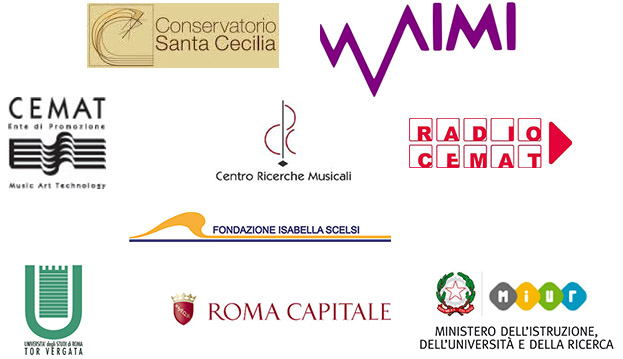
\includegraphics[width=6.4cm]{loghi.jpg}
%\caption{}
%\label{fig2_42}
\end{figure}

\end{document}